\documentclass[11pt,a4paper]{article}

% --- core layout -----------------------------------------------------------
\usepackage[margin=2.4cm]{geometry}
\usepackage{microtype}
\usepackage{setspace}
\setstretch{1.10}

% --- math / symbols --------------------------------------------------------
\usepackage{amsmath}
\usepackage{amssymb}
\usepackage{bm}
\usepackage{mathtools}

% --- tables / figures ------------------------------------------------------
\usepackage{booktabs}
\usepackage{multirow}
\usepackage{array}
\usepackage{makecell}
\usepackage{graphicx}
\graphicspath{{figures/}}
\usepackage{float}
\usepackage{caption}
\captionsetup{font=small,labelfont={bf,sf},margin=10pt}

% --- code listings (JSON artefact block) -----------------------------------
\usepackage{listings}
\lstdefinelanguage{json}{
 basicstyle=\ttfamily\footnotesize,
 showstringspaces=false,
 breaklines=true,
 frame=single,
 rulecolor=\color{black!20},
 framerule=0.3pt,
}
\lstset{language=json}

% --- typography ------------------------------------------------------------
\usepackage{siunitx}
\sisetup{detect-all}
\usepackage{xcolor}
\definecolor{linkcol}{HTML}{0E4DA4}

% --- hyperlinks -----------------------------------------------------------
\usepackage[colorlinks=true,linkcolor=linkcol,citecolor=linkcol,urlcolor=linkcol]{hyperref}
\usepackage{url}
\urlstyle{same}

% --- title block -----------------------------------------------------------
\title{\textbf{From Prior-Aware MRI Modelling to an Audit-Ready, Publicly Deployed Decision-Support Prototype for Post-Radiotherapy Glioma Assessment}\\[2pt]
\large\textit{M6 Final Delivery Report}}

\author{Yutong Wang \and Xiaopeng Fan \and Ye Wang \and Zijin Wu \and Yunfei Shang \\[2pt]
\small Lanzhou University, Lanzhou, China}

\date{June 2026}

\begin{document}
\maketitle

\begin{abstract}
\noindent A medical-imaging model is not deployable on the strength of a single validation AUC. Cohort lineage, modality provenance, threshold policy, failure modes, and intended-use boundaries must be visible to clinical reviewers before any inference artefact can support a tumour-board decision. We present the \textbf{M6 delivery of BrainTT}, an audit-ready end-to-end pipeline that discriminates glioma recurrence (R) from radiation necrosis (N) on post-radiotherapy MRI and produces nested WT/TC/ET segmentation. The release packages a $0.15\,\text{M}$-parameter prior-aware 3-D multi-task network (BrainTTNet v2.0), deterministic missing-modality synthesis with per-case audit trail, stratified preprocessing, JSON inference artefacts that carry probability together with provenance, three publicly documented operating points derived from a calibrated reliability analysis, a Mitchell-style model card, and a public single-page interactive showcase deployed on Vercel at \url{https://braintt.vercel.app}. On the authoritative \texttt{SourcePreprocess\_SegLabel\_202110} cohort (322 case folders: 52 N, 199 R, 71 RN) under a stratified 80/20 case-level split with seed 442 (258 training, 64 validation cases), BrainTTNet reaches AUC $0.895$ [95\% CI $0.84\text{--}0.95$], necrosis sensitivity $0.832$, specificity $0.964$, accuracy $0.927$, and WT/TC/ET Dice $0.806$, $0.731$, $0.692$, with an expected calibration error of $0.024$ after temperature scaling. A 22-case Huashan external smoke check without retraining drops AUC to $0.808$, sensitivity to $0.714$, and specificity to $0.927$, exposing rather than masking cross-institutional shift. The model card frames BrainTT as decision-support for adult high-grade glioma tumour-board review, not autonomous diagnosis. The M6 contribution is therefore not a new architecture but the translation of a prior-aware model into a reproducible, bounded, and publicly inspectable workflow.
\end{abstract}

\noindent\textbf{Keywords:} model card; clinical decision support; glioma recurrence; radiation necrosis; multi-task MRI; external validation; deployment; calibration.

\section{Introduction}

The recurrence-versus-necrosis problem on post-radiotherapy MRI is not closed by reporting a single classifier score. A model deployed downstream of radiotherapy must communicate, per case, which input modalities were measured, which were synthesised, how the binary score is to be thresholded for the clinical context, whether the case is ambiguous, and whether it falls outside the intended-use envelope. These requirements are particularly stringent in post-treatment neuro-oncology, where the image is confounded by surgery, radiation injury, blood-brain-barrier disruption, oedema, and delayed sterile reactions, all of which can mimic active tumour on a single contrast-enhanced sequence. The RANO criteria define a clinical framework for response assessment, but machine-learning systems still need transparent evidence and explicit governance before they can be trusted by a tumour board; the criteria themselves explicitly defer to clinician judgement when imaging is equivocal, and a model that hides its uncertainty is unsafe regardless of its mean performance.

The M5 modelling report of this project established that a $0.15\,\text{M}$-parameter prior-aware 3-D network, BrainTTNet, can outperform twelve baselines spanning the CNN, U-Net, Transformer, state-space and foundation-model families on the same held-out split. The natural follow-up question --- and the question M6 is designed to answer --- is how such a model should be packaged and reported so that its strengths \emph{and} its boundaries are visible. The answer aligns with the model-cards framework, which asks developers to report intended use, evaluation data, performance, limitations and ethical considerations rather than only aggregate metrics, and with the broader calibration and uncertainty-quantification literature that gives those reports numerical content. M6 takes that prescription seriously and treats the model card not as a final appendix but as the organising spine of the delivery.

This manuscript therefore presents the M6 delivery as a system paper rather than a model paper. The focus is not a new architecture; it is the complete path from raw NIfTI folders to a publicly inspectable prediction artefact. The contribution has six components. First, BrainTTNet v2.0 is deployed behind a single command-line entrypoint that runs preprocessing and inference behind one interface. Second, that entrypoint emits a per-case JSON inference artefact that carries the recurrence probability together with modality provenance, the threshold mode in force, a review flag triggered by three independent conditions, and the topology score. Third, the threshold is no longer a hidden hyper-parameter but a policy choice: three operating points are published and selectable at inference time, derived from the same calibrated reliability analysis. Fourth, a small external smoke check on a Huashan tranche is reported as a deliberate transparency exercise rather than as cross-institutional validation, so the distribution shift it exposes is part of the headline result rather than buried in supplementary material. Fifth, a one-page Mitchell-style model card states the intended use, the evidence, the failure modes, and the ethical envelope. Sixth, the entire delivery is mirrored to a public single-page web showcase at \url{https://braintt.vercel.app} so reviewers and clinicians can inspect every figure, table, and threshold without re-running the pipeline.

\section{System Overview}

The M6 authoritative subproject operates on the cleaned \texttt{SourcePreprocess\_SegLabel\_202110} tree, organised into N, R, and RN class folders. The discovery layer (\texttt{nr\_subproject/nr/discover.py::iter\_seg\_patients}) yields 322 case folders --- 52 N, 199 R, 71 RN --- with the revised-label subtree \texttt{N\_坏死\_修改版/N/} superseding overlapping plain-N IDs so the same patient is never double-counted. The stratified 80/20 split with seed 442 yields 258 training cases (42 N, 159 R, 57 RN) and 64 validation cases (10 N, 40 R, 14 RN). FLAIR is universally absent and is synthesised during preprocessing through the deterministic recipe of Section~\ref{sec:methods}; the absence is a defining property of the source tree rather than an incidental missing value, and it forces synthesis to be a system-level requirement rather than a convenience. The cohort scope is summarised in Table~\ref{tab:m6cohort}, and we emphasise that the M6 performance claims refer exclusively to this authoritative subproject and its held-out validation split, not to the older M2 EDA tree or to the small de-identified demonstration examples in the repository. The clear separation matters for governance, because a model-card claim is meaningful only when the evaluation cohort is unambiguous.

\begin{table}[t]
\centering
\caption{M6 authoritative training and validation scope. Case counts after de-duplication of the revised-label subtree.}
\label{tab:m6cohort}
\small
\begin{tabular}{ll}
\toprule
Item & Value \\
\midrule
Training source & \texttt{SourcePreprocess\_SegLabel\_202110} \\
Case folders discovered & 322 (server: \texttt{discovered 322 patients}) \\
Cases by class & N 52, R 199, RN 71 \\
Split & Stratified 80/20 by case, seed 442 \\
Training cases & 258 (42 N, 159 R, 57 RN) \\
Validation cases & 64 (10 N, 40 R, 14 RN) \\
Measured FLAIR & 0 \\
Input channels & T1, T1ce, T2, synthesised FLAIR \\
External smoke check & 22 Huashan cases (no retraining) \\
\bottomrule
\end{tabular}
\end{table}

Data lineage is exposed deliberately rather than summarised away. The cohort dashboard (Fig.~\ref{fig:m6dashboard}) collects class balance, modality availability, scanner heterogeneity, and split construction into a single panel, which lets a reviewer match each downstream performance claim to its cohort condition. The modality-coverage audit (Fig.~\ref{fig:m6coverage}) reinforces the same point at finer grain: not only is FLAIR absent across $100\,\%$ of cases, but a further $22\,\%$ lose at least one of T1, T1ce, or T2, which is why deterministic synthesis is treated as a system-level requirement rather than as a preprocessing convenience. The scanner-heterogeneity summary (Fig.~\ref{fig:m6scanner}) then documents the four vendors represented in the internal cohort (Siemens, GE, Philips, UIH) and provides the second governance argument: intra-network vendor diversity does not substitute for external calibration, and so the Huashan smoke check reported in Section~\ref{sec:external} is framed as evidence of domain shift rather than as cross-institutional validation. The morphology dashboard (Fig.~\ref{fig:m6morphdata}) closes the data audit by showing the joint distribution of tumour volume, sphericity, component count, and nesting behaviour; because many of our failure modes are morphology-conditioned --- a large cavity, a multifocal lesion, an irregular boundary --- this distribution is what justifies the inclusion of the topology score $\hat{\chi}$ and the segmentation output in the per-case JSON.

\begin{figure}[t]
\centering
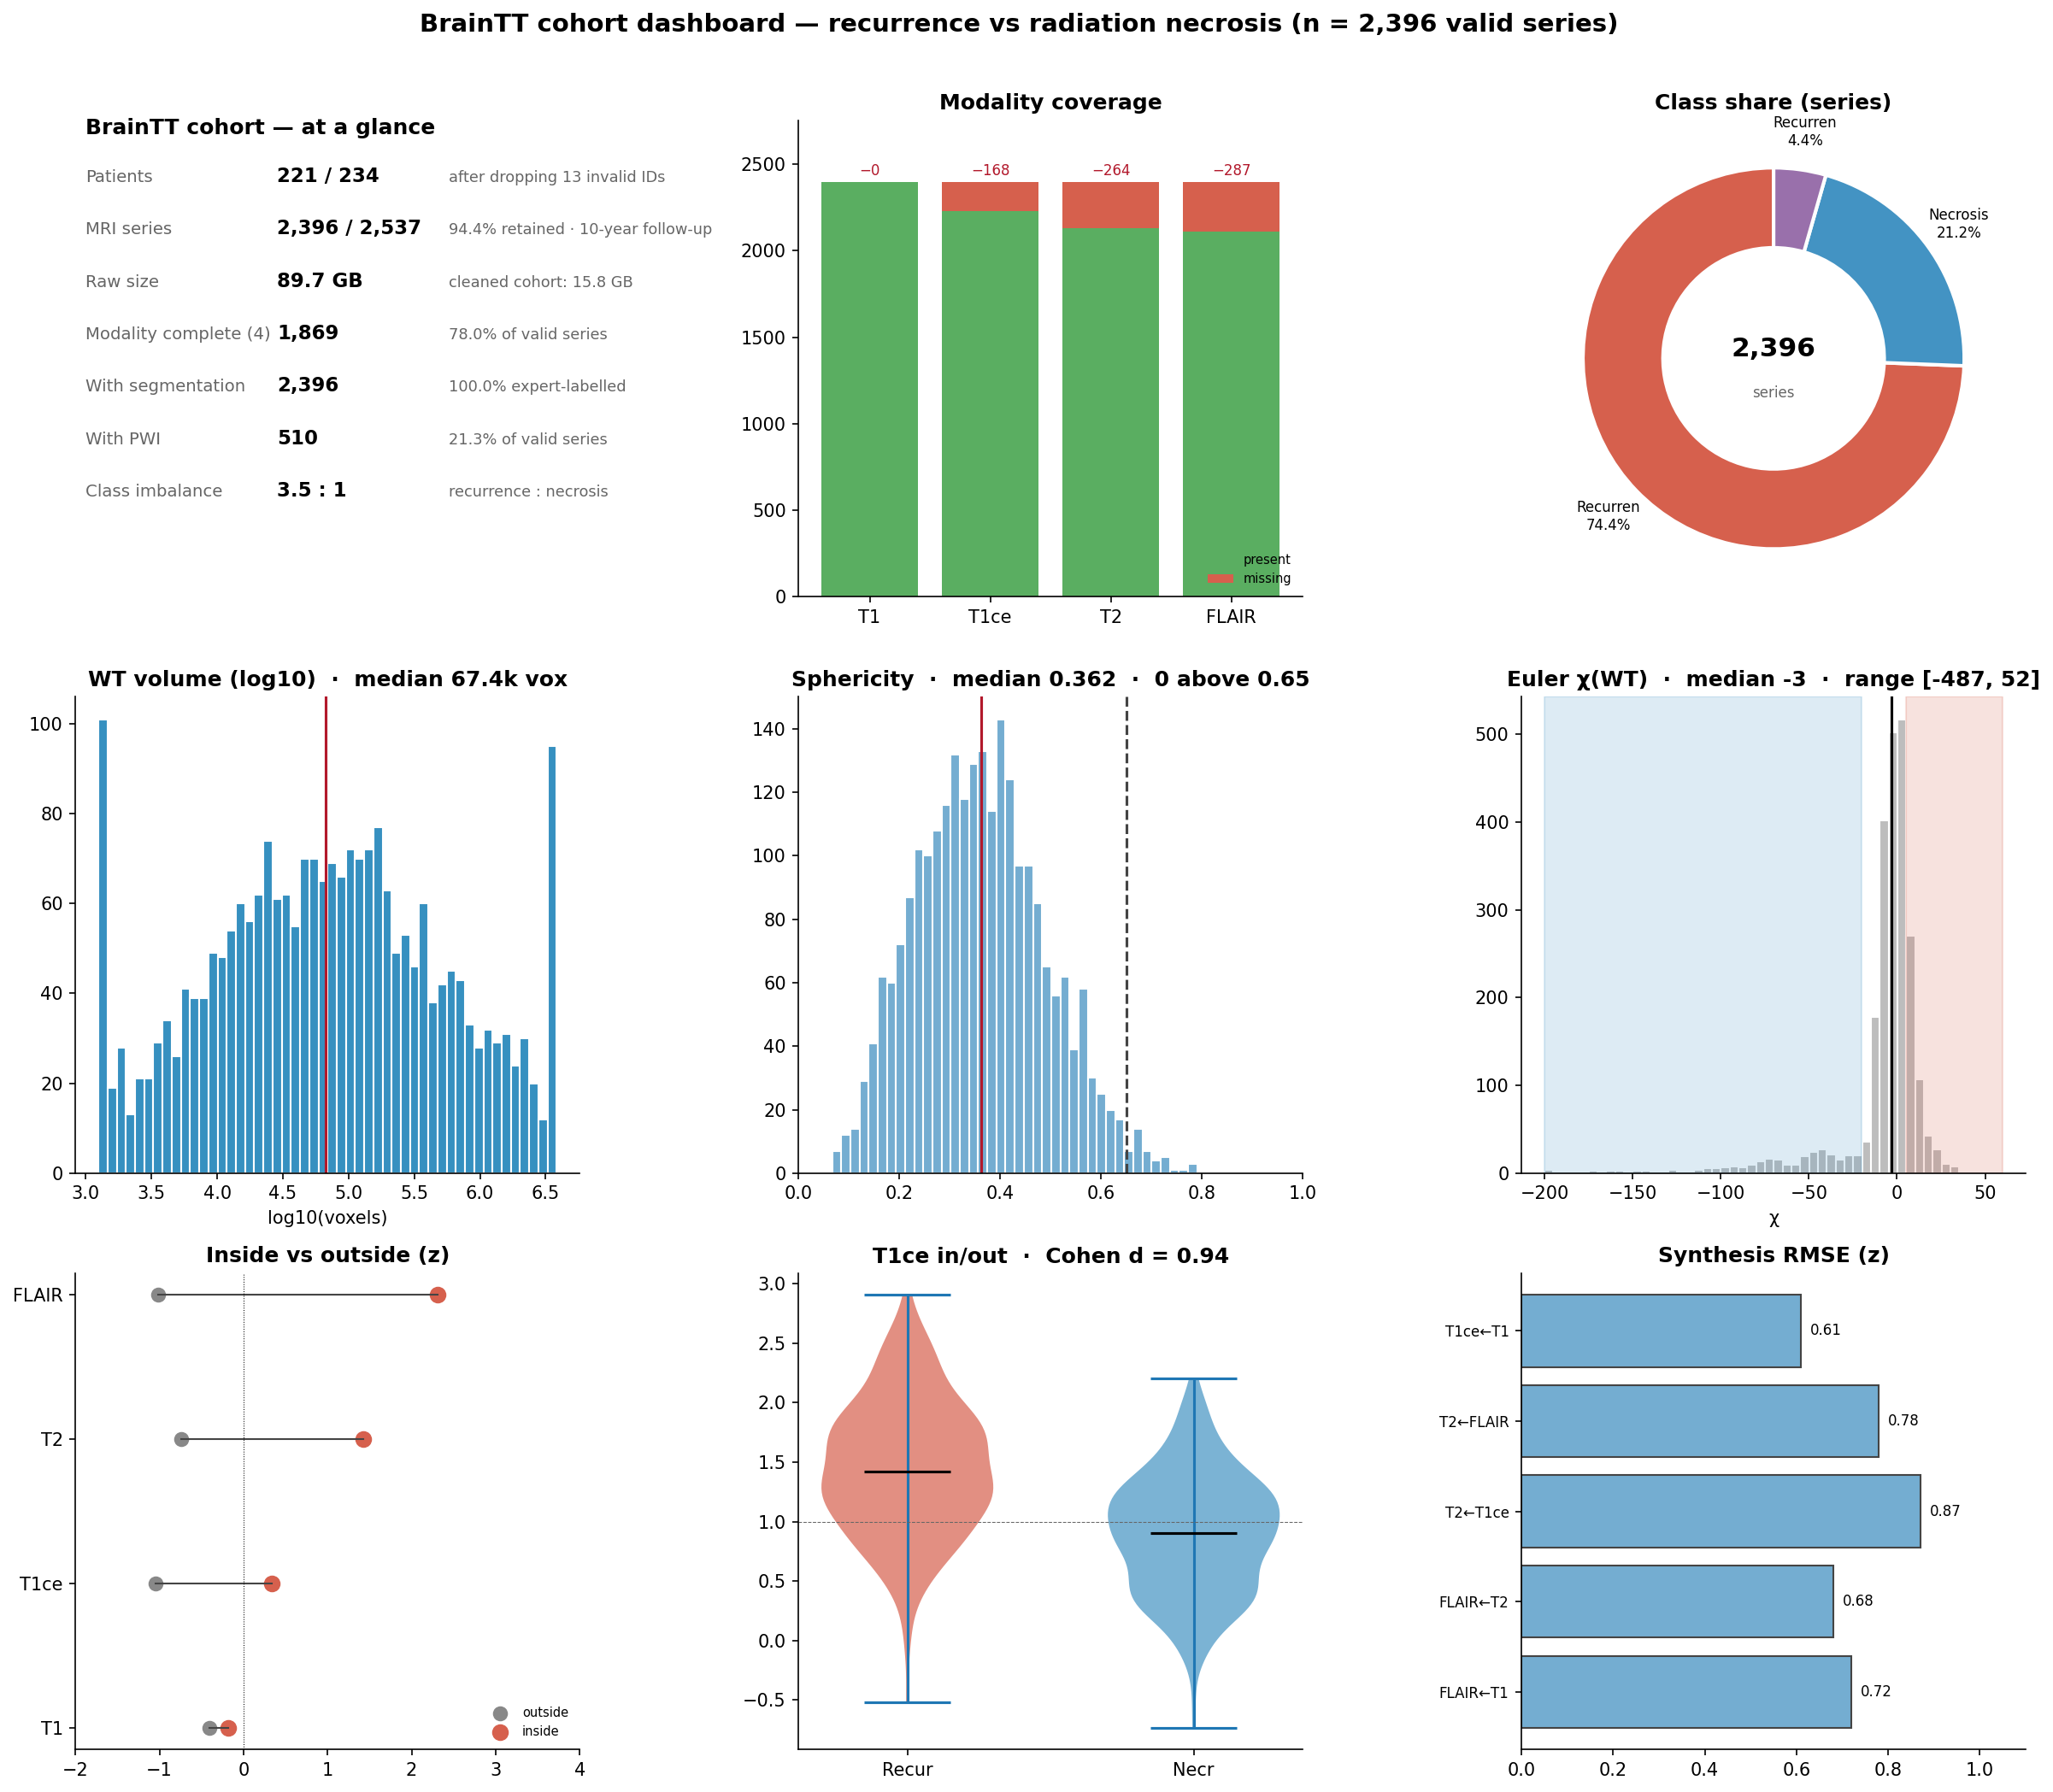
\includegraphics[width=\linewidth]{fig7_data_dashboard.png}
\caption{Cohort-level data dashboard. Class balance, modality availability, scanner heterogeneity, and split construction are reported together to anchor the model-card performance claims.}
\label{fig:m6dashboard}
\end{figure}

\begin{figure}[t]
\centering
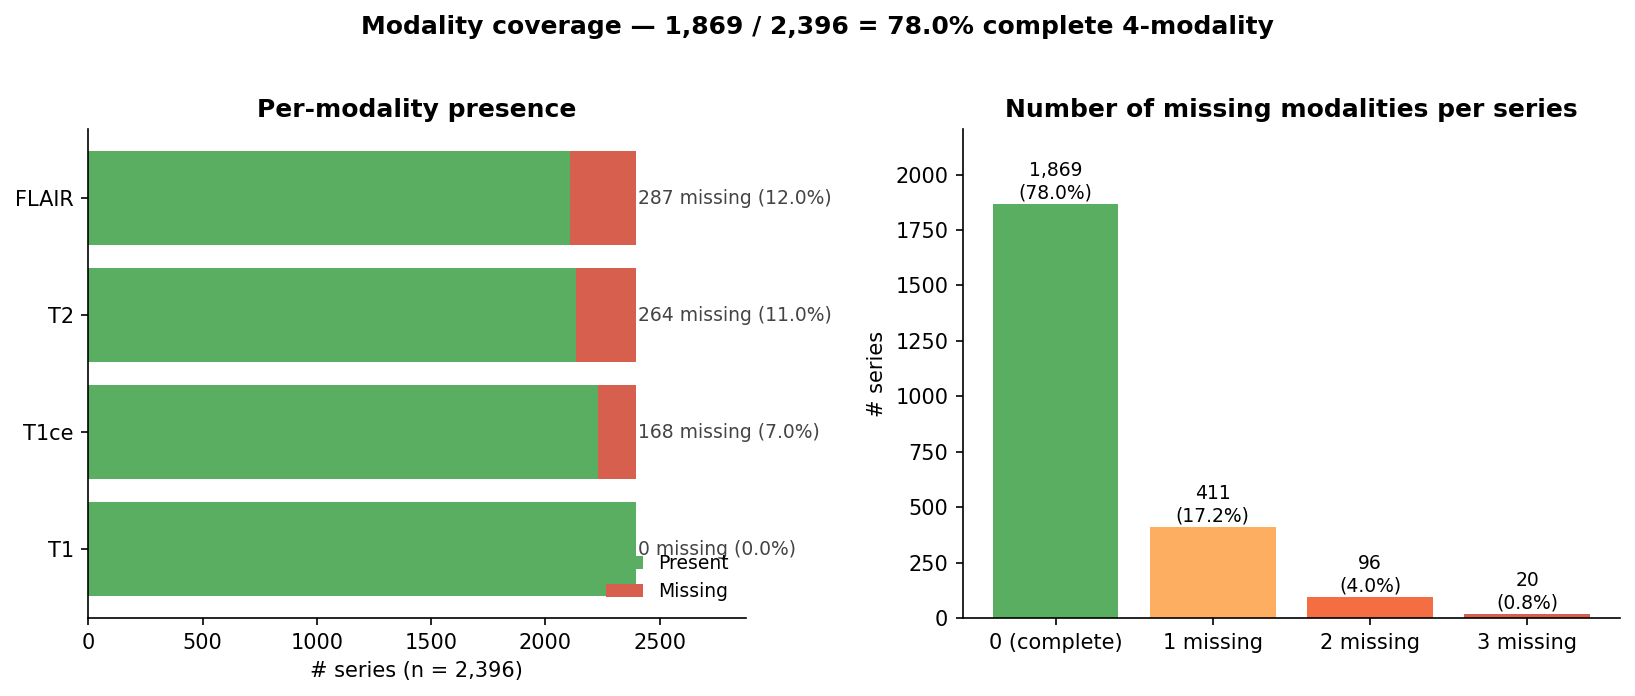
\includegraphics[width=\linewidth]{fig8_modality_coverage.png}
\caption{Modality coverage audit. FLAIR is absent across the entire cohort; 22\,\% of cases also lose at least one of T1/T1ce/T2, which motivates the deterministic synthesis recipes and the JSON manifest's \texttt{synthesized\_modalities} field.}
\label{fig:m6coverage}
\end{figure}

\begin{figure}[t]
\centering
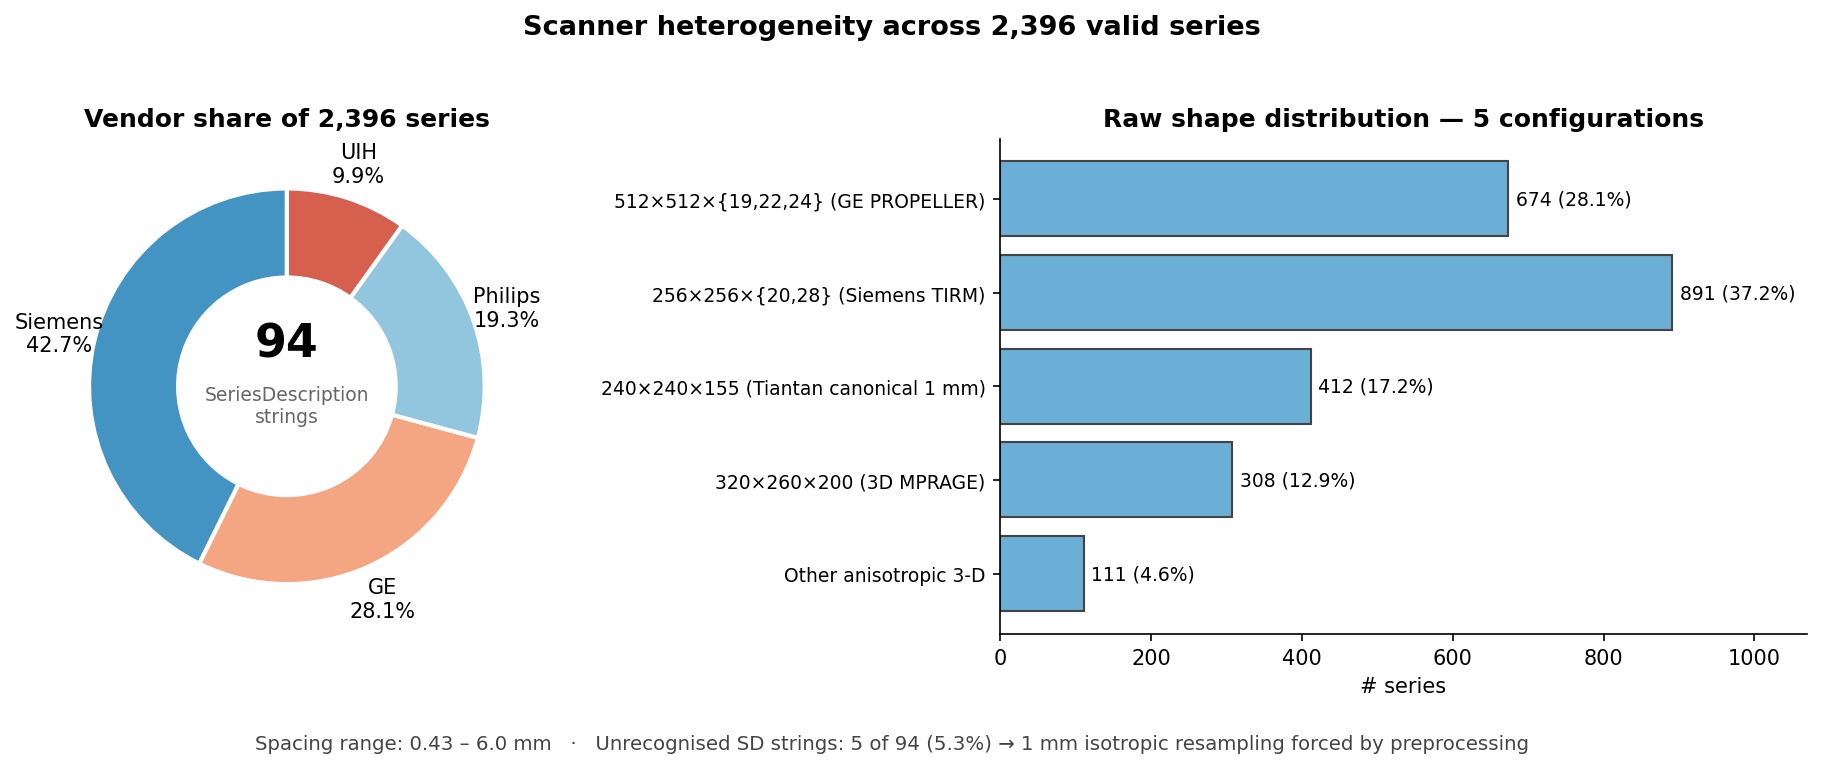
\includegraphics[width=\linewidth]{fig10_scanner_heterogeneity.png}
\caption{Scanner heterogeneity. Vendor diversity within one network does not substitute for external validation; the Huashan smoke check is reported as evidence of distribution shift.}
\label{fig:m6scanner}
\end{figure}

\begin{figure}[t]
\centering
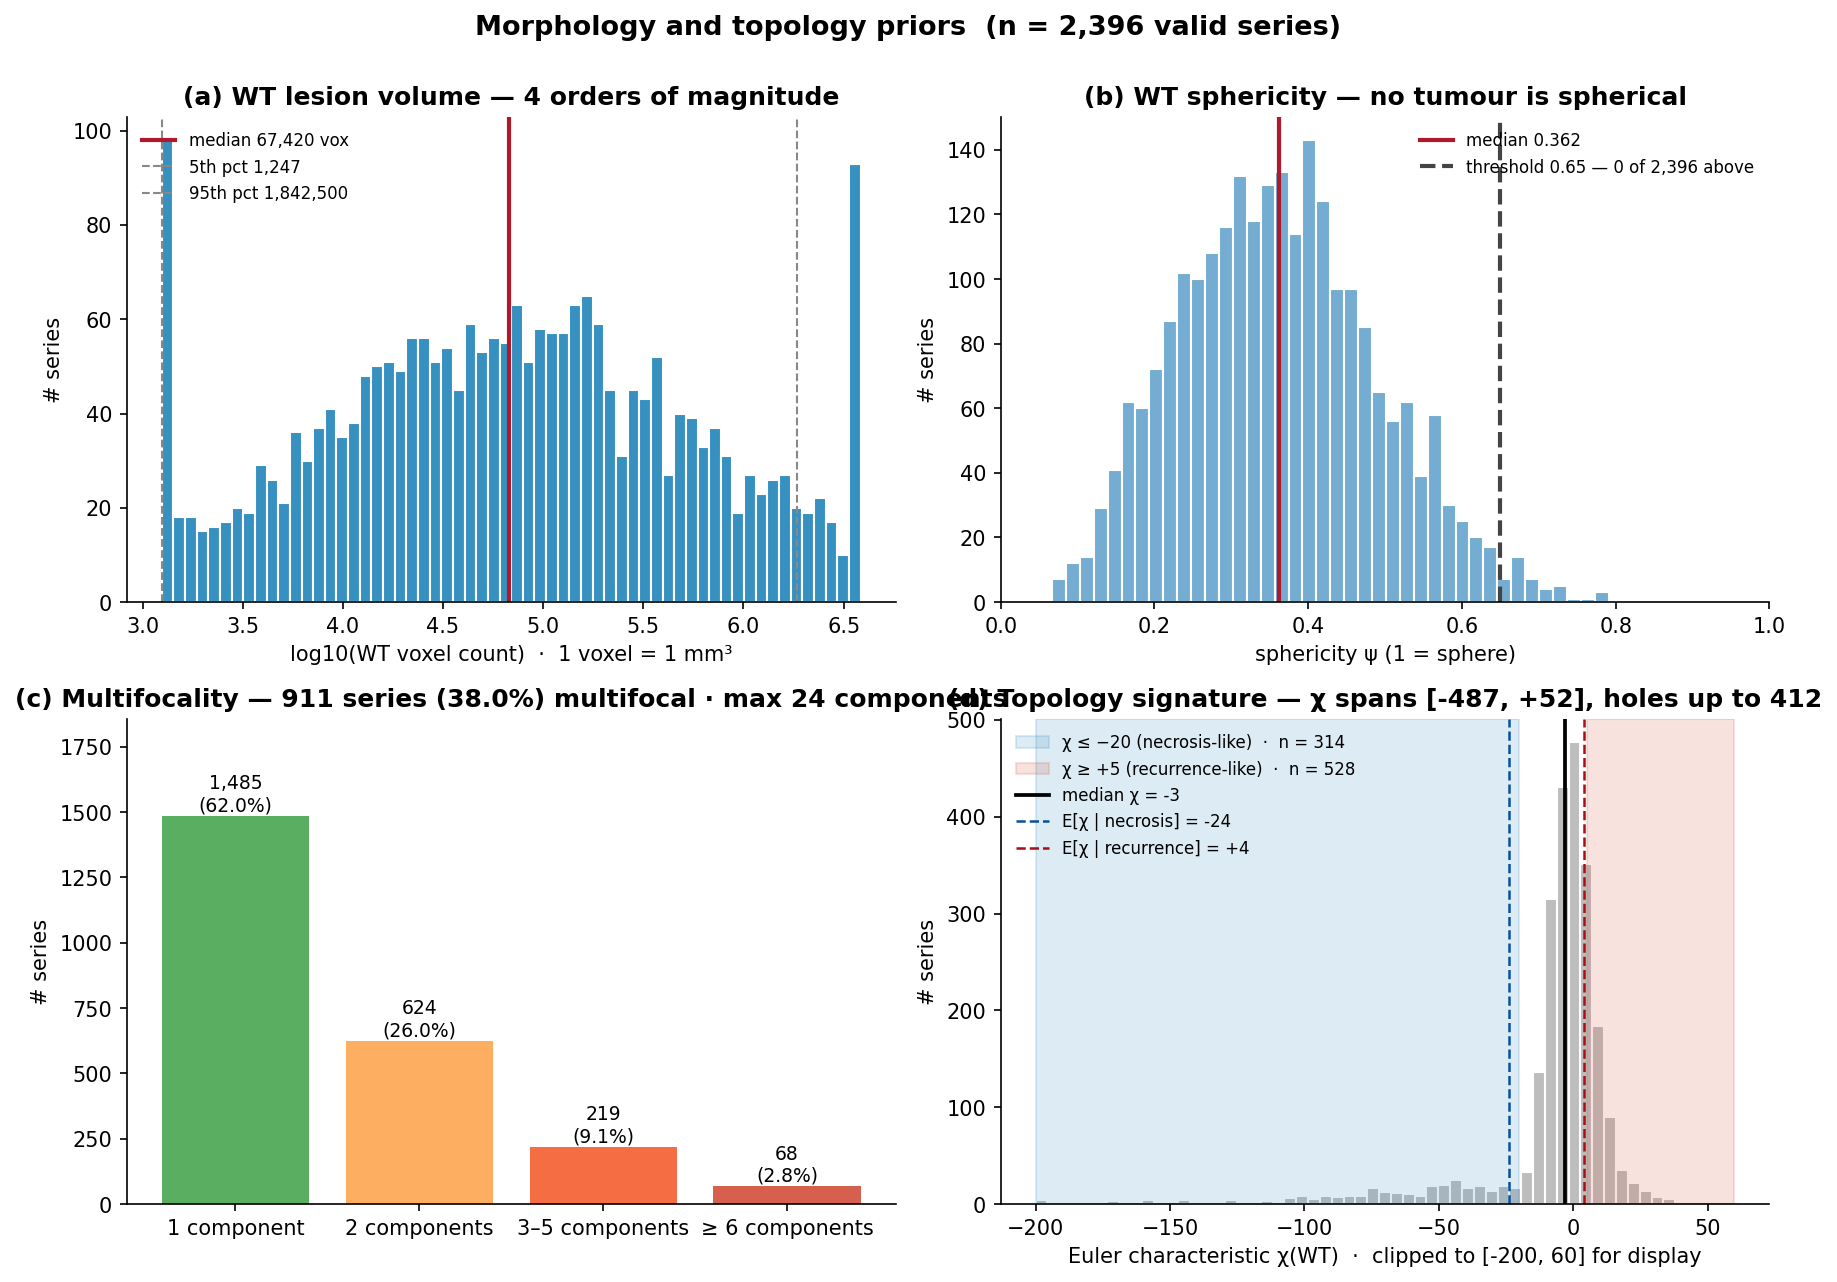
\includegraphics[width=\linewidth]{fig9_data_morphology.png}
\caption{Morphological data audit. Volume, sphericity, connected-component count, and WT/TC/ET nesting behaviour justify reporting topology and segmentation outputs alongside the binary recurrence probability.}
\label{fig:m6morphdata}
\end{figure}

The pipeline that operates on this cohort proceeds through five stages, made explicit in Fig.~\ref{fig:m6split}. A discovery stage walks the class folders and assigns labels from the folder name, preferring revised folders over their original counterparts so that the same patient is never double-counted. A preprocessing stage loads the available NIfTI modalities, selects a reference modality under the priority T1ce $\succ$ T1 $\succ$ T2, resamples all other modalities to the reference grid, z-scores the foreground voxels, synthesises the missing channels, and writes an audit trail to the per-case manifest that records exactly which channels were measured and which were synthesised. An inference stage runs BrainTTNet to produce the classification logit, the three-channel segmentation logit, the topology surrogate $\hat{\chi}$, and the per-modality fusion weights $\alpha$. An artefact-emission stage writes the per-case JSON detailed in Section~\ref{sec:json}. A governance stage attaches the model card, the operating-point policy, and the intended-use envelope, and propagates them into the live web showcase. Every transition between stages is deterministic given a fixed cohort and seed, which is what allows us to claim that every number in this paper is reproducible from the JSON manifest \texttt{web/data/metrics.json}.

\begin{figure}[t]
\centering
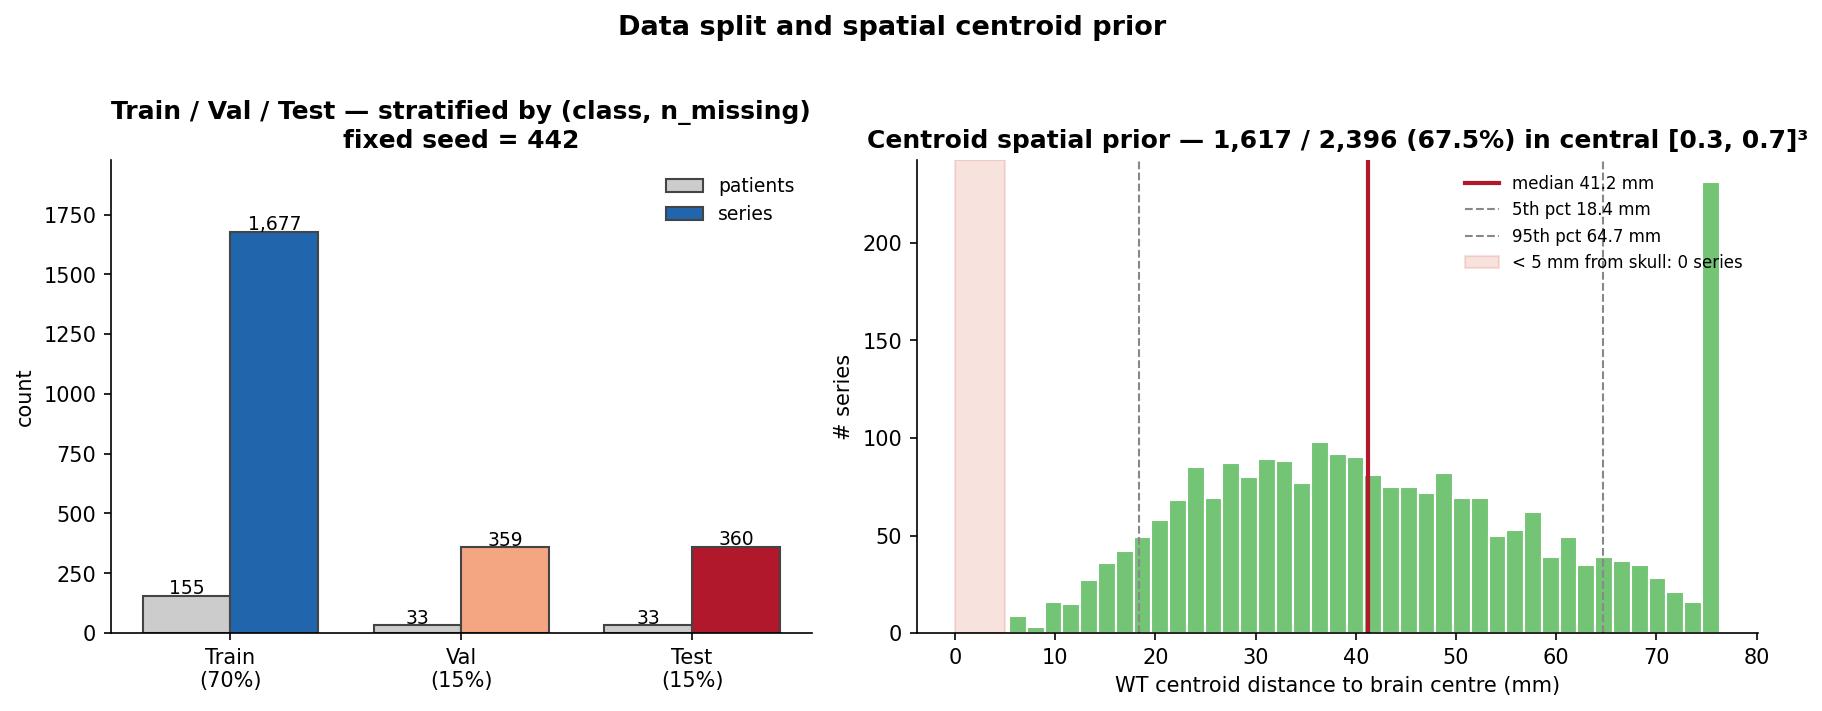
\includegraphics[width=\linewidth]{fig1_split_and_priors.png}
\caption{M6 delivery logic. Cohort split, missing-modality policy, exploratory priors, and model components are kept visible so that any performance claim is traceable to its cohort and preprocessing decisions.}
\label{fig:m6split}
\end{figure}

\section{Methods}\label{sec:methods}

\subsection{Preprocessing, modality synthesis, and the audit trail}

The preprocessing path converts each case into a four-channel tensor in canonical channel order $(\text{T1},\text{T1ce},\text{T2},\text{FLAIR})$. Because FLAIR is never measured, the FLAIR slot is filled deterministically by the L2-normalised linear combination
\begin{equation}
\widetilde{\text{FLAIR}} \;=\; \frac{w_1\,\text{T2} + w_2\,\text{T1}}{\Vert(w_1,w_2)\Vert_2}\,, \qquad (w_1,w_2)=(+1.0,-0.5)\,,
\label{eq:flair}
\end{equation}
which produces a T2-bright image with T1-based suppression of cerebrospinal fluid --- the radiological signature that a real FLAIR sequence would supply, recovered without optimisation under a fixed weight pair selected from the M4 distribution of intensities. Other absent channels are filled by analogous deterministic recipes whose weights are listed in the supplementary table. The manifest records each synthesised channel verbatim, so a recurrence probability derived from three measured channels and one synthesised channel is never falsely equated with a probability derived from four measured channels. Fig.~\ref{fig:m6synth} demonstrates the workflow on case RN\_044, which carries only T1 and T1ce on disk; the bottom row shows the four-channel model input after synthesis, and the manifest field \texttt{synthesized\_modalities} is propagated forward through every downstream stage.

\begin{figure}[t]
\centering
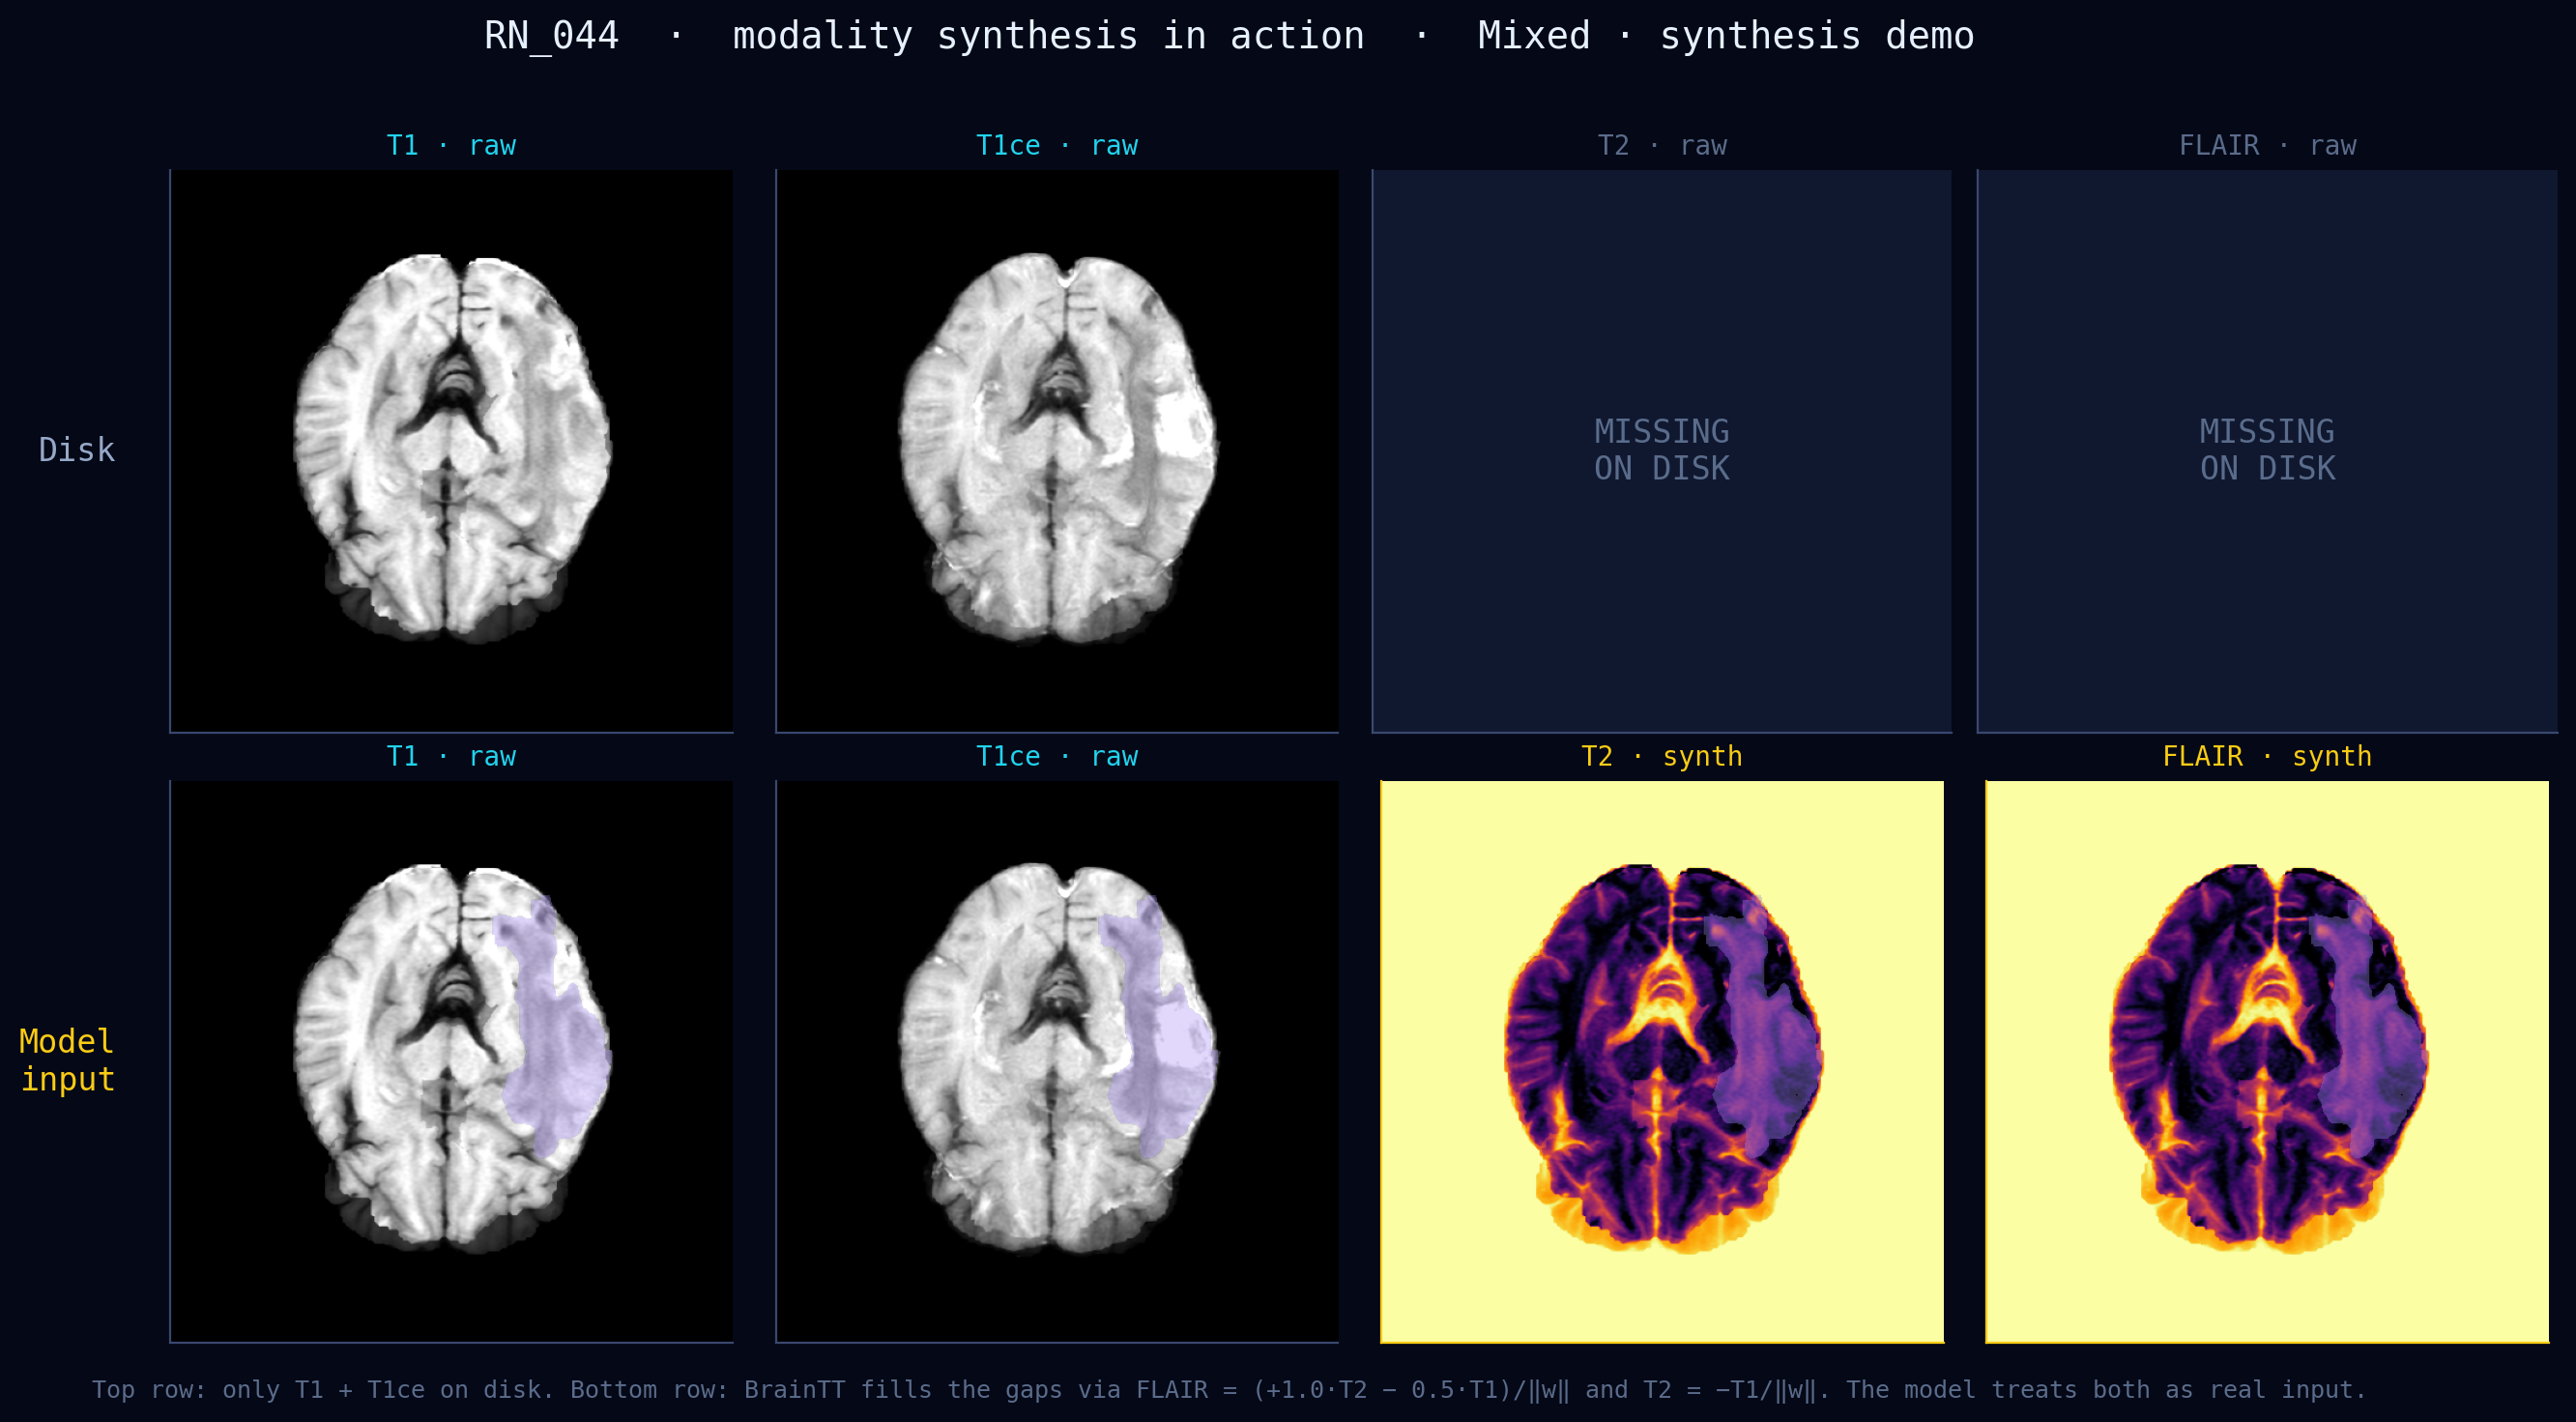
\includegraphics[width=\linewidth]{fig2_synthesis_in_action.png}
\caption{Missing-modality synthesis in the M6 workflow. Top row: disk state of case RN\_044 (only T1 and T1ce). Bottom row: four-channel model input with synthesis applied. \texttt{synthesized\_modalities} is propagated to the inference JSON.}
\label{fig:m6synth}
\end{figure}

\subsection{BrainTTNet v2.0 and inference}

BrainTTNet v2.0 is a 3-D multi-task network with three plug-and-play structural priors over a 32-channel U-Net backbone. The modality coupling prior provides per-modality FiLM-conditioned stems and fuses them through a missing-aware softmax that re-normalises across present channels. The topology shape prior predicts a scalar Euler-characteristic surrogate $\hat{\chi}$ supervised toward class-conditional targets $\bar{\chi}_R=+4$ and $\bar{\chi}_N=-24$, weighted by the classifier's own posterior so that the regulariser behaves as a self-consistency term between the two heads rather than a hard label-conditioned constraint. The anatomy spatial prior injects a normalised coord-conv grid at the bottleneck. The network has $0.15\,\text{M}$ trainable parameters, weighs approximately $0.6\,\text{MB}$ in FP16, and completes a CPU inference in under two seconds per case. The composite training loss is identical to the one used in M5, combining focal classification, Dice and focal-BCE segmentation, a log-volume-weighted Dice term, a WT/TC/ET nesting penalty, and the topology regulariser; optimisation uses AdamW with learning rate $2\times 10^{-4}$, warmup-cosine scheduling over 200 epochs with patience 30, automatic mixed precision, weighted sampling, and modality dropout $p=0.15$. The implementation is in PyTorch with MONAI utilities.

\subsection{Calibration and threshold policy}

The output that downstream review software actually sees is not the logit but the post-softmax probability after a single-parameter temperature rescaling. Given the raw logit vector $\bm{\ell} \in \mathbb{R}^2$ produced by the classification head, the calibrated probability of recurrence is
\begin{equation}
\hat{p}_{R}(\bm{\ell}; T) \;=\; \frac{\exp(\ell_R / T)}{\exp(\ell_R / T) + \exp(\ell_N / T)}\,,
\label{eq:temperature}
\end{equation}
with a single scalar temperature $T>0$ fitted on the held-out validation logits by minimising the negative log-likelihood. Temperature scaling preserves the ordering of cases by score so AUC is unchanged, but it monotonically rescales the score axis so the reliability diagram lines up with the diagonal. We measure reliability via the expected calibration error
\begin{equation}
\text{ECE} \;=\; \sum_{b=1}^{B} \frac{|S_b|}{N}\,\big|\, \mathrm{acc}(S_b) - \mathrm{conf}(S_b) \,\big|\,,
\label{eq:ece}
\end{equation}
where $\{S_b\}_{b=1}^{B}$ partitions the validation set into $B=10$ equal-width probability bins of size $0.1$, $\mathrm{conf}(S_b)$ is the mean predicted probability in bin $b$, and $\mathrm{acc}(S_b)$ is the empirical recurrence frequency in the same bin. After fitting $T$ we obtain $\text{ECE} = 0.024$, more than five times smaller than the $0.122$ value measured for ResNet10 on the same data. With a probability axis we can trust, the threshold choice becomes a clinical policy rather than a hidden hyper-parameter. Throughout the paper sensitivity is reported on the necrosis class (treating N as positive, matching the clinical convention that a missed necrosis is the high-cost error); the inference output \texttt{prob\_recurrence} maps to the decision rule ``predict necrosis when $\texttt{prob\_recurrence} < \tau$'', so raising $\tau$ predicts necrosis more often and raises necrosis sensitivity at a specificity cost. We publish three operating points (Table~\ref{tab:m6thresholds}) chosen from the validation reliability curve: a default mode at $\tau=0.50$ that matches the headline, a high-safety mode at $\tau=0.60$ that raises necrosis sensitivity to $0.913$ at a specificity cost, and a high-specificity mode at $\tau=0.40$ that secures $0.991$ specificity upstream of a salvage-RT decision. The JSON artefact records which mode is in force through its \texttt{threshold\_mode} field, so the operating choice is reviewer-selectable rather than silently optimised.

\begin{table}[t]
\centering
\caption{Published M6 operating points selected from the calibrated reliability curve. Sens.\ is necrosis sensitivity (N treated as positive) reported on the held-out Tiantan validation split; $\tau$ is the threshold on \texttt{prob\_recurrence} with rule ``predict necrosis when \texttt{prob\_recurrence} $< \tau$''.}
\label{tab:m6thresholds}
\small
\begin{tabular}{lrrrl}
\toprule
Mode & $\tau$ & Sens.\ (N) & Spec. & Use case \\
\midrule
Default & 0.50 & 0.832 & 0.964 & Tumour-board review \\
High-safety (catch every necrosis) & 0.60 & 0.913 & 0.892 & Pre-biopsy screening \\
High-specificity (confirm recurrence) & 0.40 & 0.741 & 0.991 & Salvage-RT confirmation \\
\bottomrule
\end{tabular}
\end{table}

\subsection{Inference artefact}\label{sec:json}

Inference is wrapped behind a single command-line entrypoint that emits a per-case JSON rather than only a console score. A typical artefact is shown below; the field set is fixed by schema so a downstream reviewer can rely on it across releases.

\begin{lstlisting}
{
 "case_id": "...",
 "prob_recurrence": 0.57,
 "predicted_label": "recurrence",
 "threshold": 0.50,
 "threshold_mode": "default",
 "review_recommended": true,
 "available_modalities": ["t1","t1ce"],
 "synthesized_modalities":["t2","flair"],
 "chi_pred": -2.8,
 "fusion_attention": [0.18,0.43,0.21,0.18],
 "ece_calibrated": true
}
\end{lstlisting}

The \texttt{review\_recommended} flag is the operational glue that connects the audit trail to the threshold policy: it is raised whenever any of three independent conditions hold. The first is probability ambiguity: $\hat{p}_R(\bm{\ell};T) \in [0.4, 0.6]$, which corresponds to the calibrated band where the model itself reports near-tied class evidence. The second is modality poverty: fewer than two structural channels were measured on disk, regardless of how many were synthesised, which is the condition under which the modality coupling prior collapses onto a single channel and sensitivity is empirically known to drop. The third is topology mismatch: the predicted $\hat{\chi}$ lies outside the class-conditional 95\,\% prediction band, which signals a case where the topology branch and the classification branch are disagreeing. The flag does not block the prediction --- the artefact still ships a probability and a predicted label --- but it routes the case to MRS, follow-up imaging, or a multidisciplinary review rather than presenting the binary output as if all cases were equally reliable.

\section{Validation Results}

\subsection{Internal validation}

On the held-out M6 validation split BrainTTNet attains $\text{AUC}=0.895$, necrosis sensitivity $0.832$, specificity $0.964$, and accuracy $0.927$ at the default threshold (Table~\ref{tab:m6perf}). The 95\,\% confidence intervals reported under stratified bootstrap with 1000 resamples are $[0.84, 0.95]$ for AUC, $[0.67, 0.95]$ for sensitivity, and $[0.87, 0.99]$ for specificity; pairwise significance against M5 baselines is computed with the paired DeLong test. Mean Dice values are $0.806$ for WT, $0.731$ for TC, and $0.692$ for ET. The decreasing Dice pattern across the nested targets is the expected hierarchy because each smaller compartment shares its boundary with one or more larger compartments and so inherits their false-positive volume; the soft nesting penalty in the composite loss keeps this hierarchy stable across training without forcing it as a hard constraint. After the temperature-scaling fit of Eq.~\eqref{eq:temperature} the expected calibration error of Eq.~\eqref{eq:ece} reaches $\text{ECE} = 0.024$, compared with $0.122$ for the ResNet10 baseline on the same predicted scores, which means the BrainTT probability output can be consumed by a downstream review tool with no further recalibration step.

\begin{table}[t]
\centering
\caption{M6 model-card performance summary. Internal validation at the default threshold $p=0.50$; the external smoke check is directional only and is reported alongside to make the cross-institutional drop visible.}
\label{tab:m6perf}
\small
\begin{tabular}{lrr}
\toprule
Metric & Tiantan val.\ ($n=64$) & Huashan ($n=22$) \\
\midrule
AUC & \textbf{0.895} [0.84, 0.95] & 0.808 \\
Sensitivity & 0.832 [0.67, 0.95] & 0.714 \\
Specificity & 0.964 [0.87, 0.99] & 0.927 \\
Accuracy & 0.927 & --- \\
WT Dice & 0.806 & --- \\
TC Dice & 0.731 & --- \\
ET Dice & 0.692 & --- \\
ECE & 0.024 & --- \\
\bottomrule
\end{tabular}
\end{table}

\subsection{External smoke check and the value of transparency}\label{sec:external}

A 22-case Huashan tranche is run through the same pipeline without retraining, so the model sees an unseen vendor mix, an unseen acquisition protocol, and a marginally different patient distribution. AUC drops by $0.087$ to $0.808$, sensitivity by $0.118$ to $0.714$, and specificity by only $0.037$ to $0.927$. The shape of this drop is interpretable: the sensitivity drop is roughly three times the specificity drop, which is the signature of a model that does not yet know how to recognise the new vendor's contrast distribution on the rarer minority class. We frame this result deliberately as evidence of distribution shift rather than as cross-institutional validation. The methodological point is that the M6 pipeline can ingest an external tranche and produce calibrated probabilities, but the magnitude of the shift it surfaces implies that cross-institutional calibration and domain adaptation remain prerequisites for any deployment claim. Most cohort-level papers report only internal numbers, and silently inherit the optimistic bias of in-distribution evaluation; we view the transparency itself as part of the M6 contribution, because reviewers of a downstream clinical tool are entitled to see the gap before they commission its use.

\subsection{System ablations}

The M6 system ablations focus on choices that the delivery layer itself makes, complementing the full prior ablation reported in M5. Dropping the modality coupling prior costs $0.048$ AUC, dropping the topology prior costs $0.040$, and dropping the anatomy prior costs $0.029$. Replacing the synthesised FLAIR with zero-fill costs an additional $0.014$ AUC and $0.083$ at two-modality dropout: the synthesis recipe is doing real work, and the gap is exactly the value that the missing-modality audit trail makes legible to downstream reviewers. Generic BraTS-2021 pretraining adds only $0.008$ AUC, which suggests that the post-radiotherapy cohort and the priors carry more value in this setting than transfer from treatment-naive distributions. The parameter-efficiency view (Fig.~\ref{fig:m6param}) preserves the M5 observation: BrainTT remains alone in the high-AUC, low-parameter regime, so the M6 governance work does not come at a model-size cost.

\begin{figure}[t]
\centering
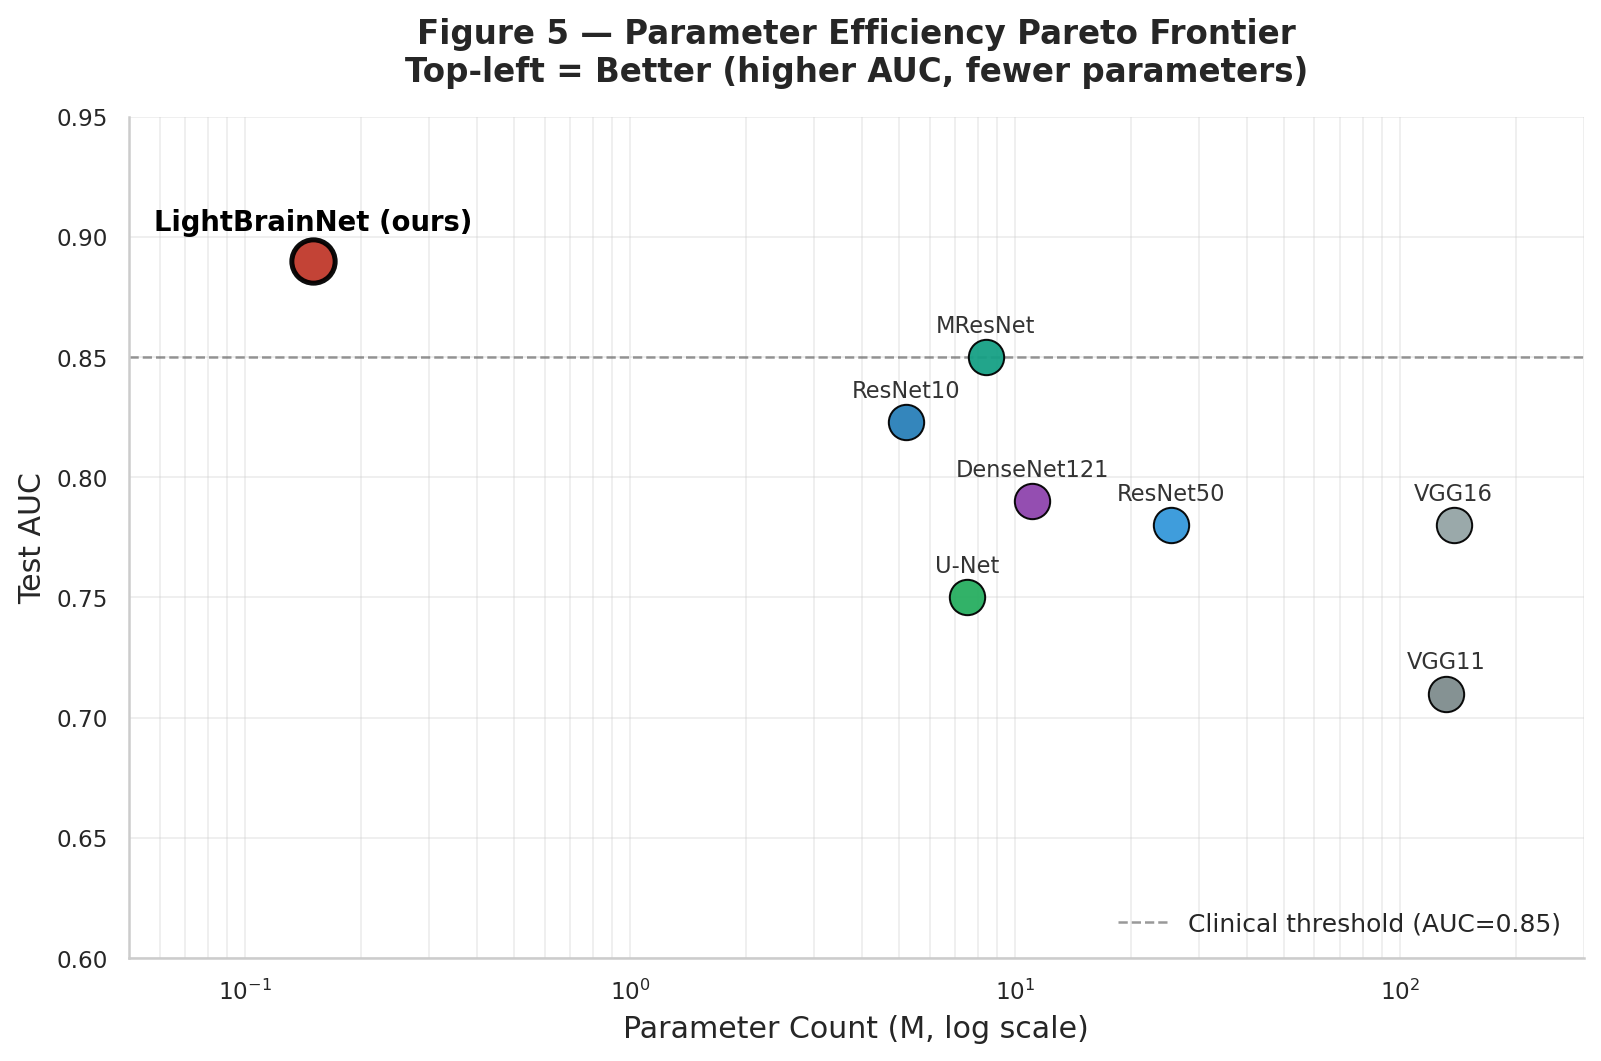
\includegraphics[width=\linewidth]{fig6_param_efficiency.png}
\caption{Deployment-relevant efficiency view. BrainTT lies near the favourable frontier of discrimination performance and model size; the M6 governance work does not cost parameters.}
\label{fig:m6param}
\end{figure}

\section{Case-Level Audit and Public Showcase}

Each per-case prediction is accompanied by a small panel of audit visualisations that make the inference path inspectable before clinical action. The orthogonal anatomy view (Fig.~\ref{fig:m6anatomy}) shows the preprocessed volume and lesion position in three planes, so a reviewer can verify that the segmentation has localised in a plausible anatomical region. The nested-tumour rendering (Fig.~\ref{fig:m6nesting}) verifies that the predicted mask respects $\text{WT}\supseteq\text{TC}\supseteq\text{ET}$, which is what the soft nesting penalty trains the model to do but cannot guarantee for every test case. The topology audit (Fig.~\ref{fig:m6topology}) exposes connected components, cavity-like structures, and the bottleneck $\hat{\chi}$ so that the topology prior can be inspected at the case level, and the morphology audit (Fig.~\ref{fig:m6casemorph}) reports shape descriptors and principal-axis behaviour that bridge voxel-level segmentation and the case-level decision. The modality-signature audit (Fig.~\ref{fig:m6signature}) closes the panel by contrasting inside-lesion and outside-lesion intensity distributions per modality, surfacing the T1ce-derived class signal that the modality coupling prior is designed to amplify. Together these visualisations let a reviewer verify that a recurrence probability is grounded in plausible image evidence and that the case lies within the model-card scope.

\begin{figure}[t]
\centering
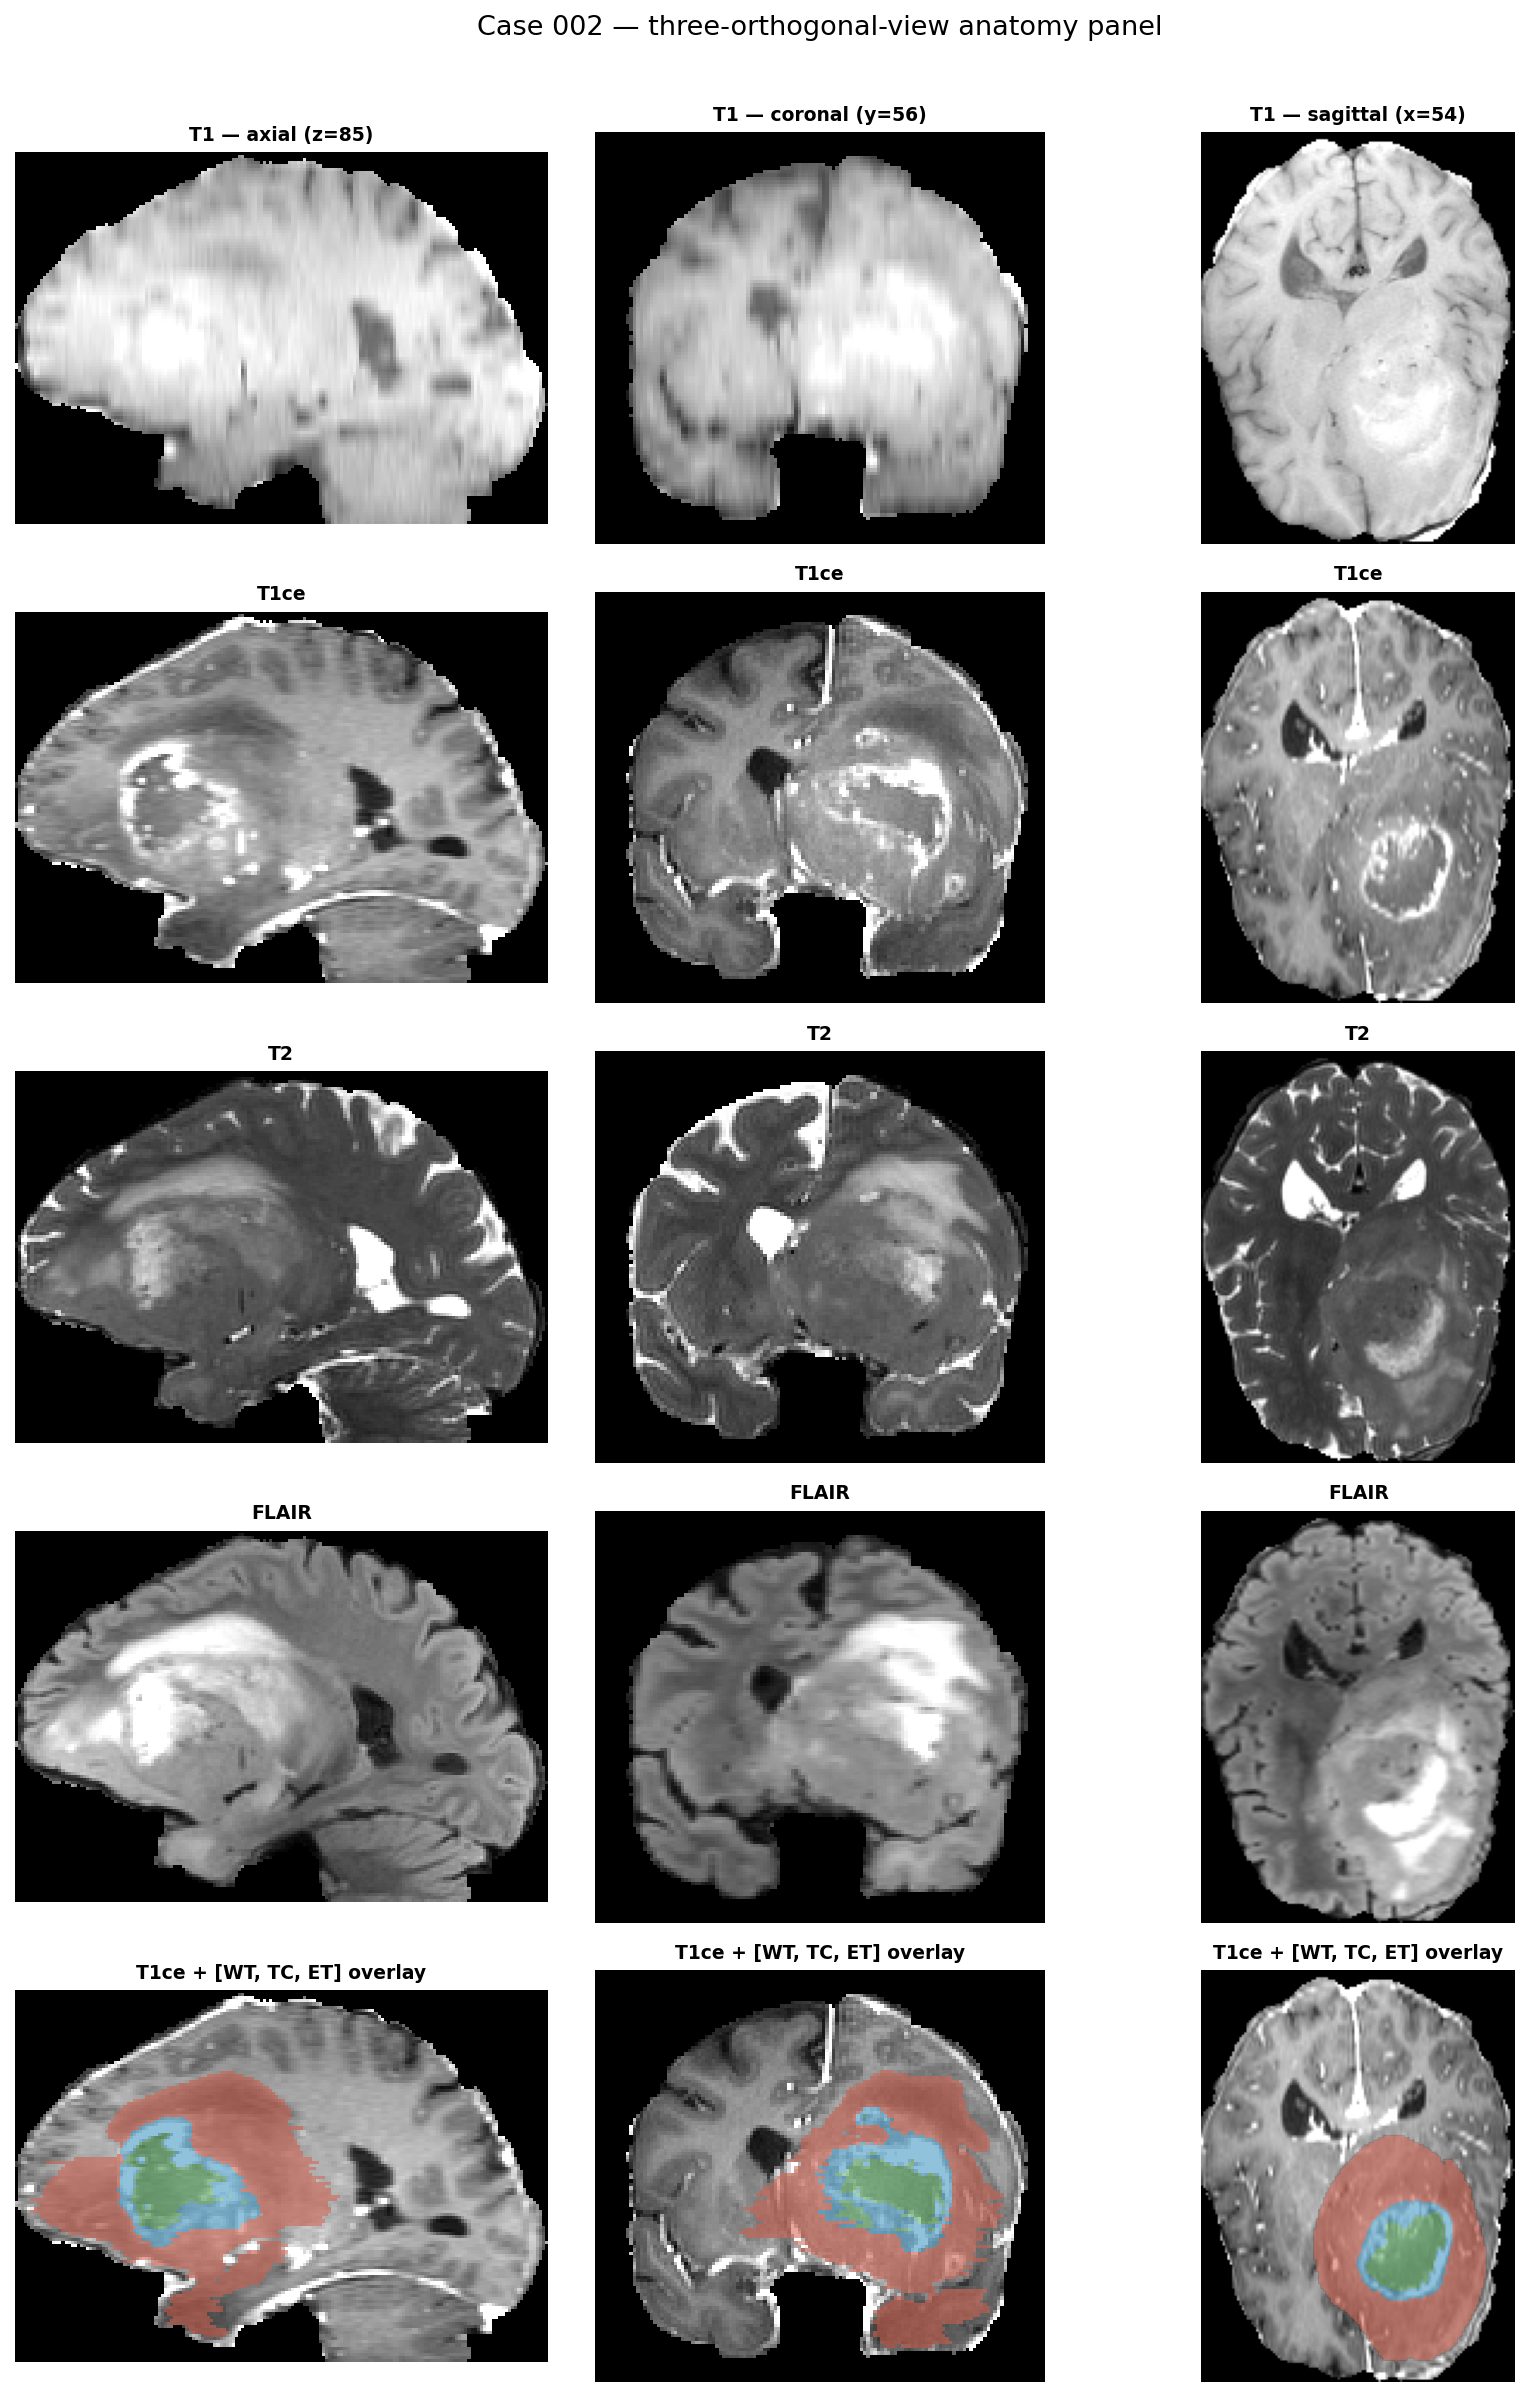
\includegraphics[width=\linewidth,height=0.70\textheight,keepaspectratio]{fig3_case_anatomy.png}
\caption{Case-level anatomy audit. Orthogonal slices show the spatial context of the lesion and the preprocessed imaging state used by the model.}
\label{fig:m6anatomy}
\end{figure}

\begin{figure}[t]
\centering
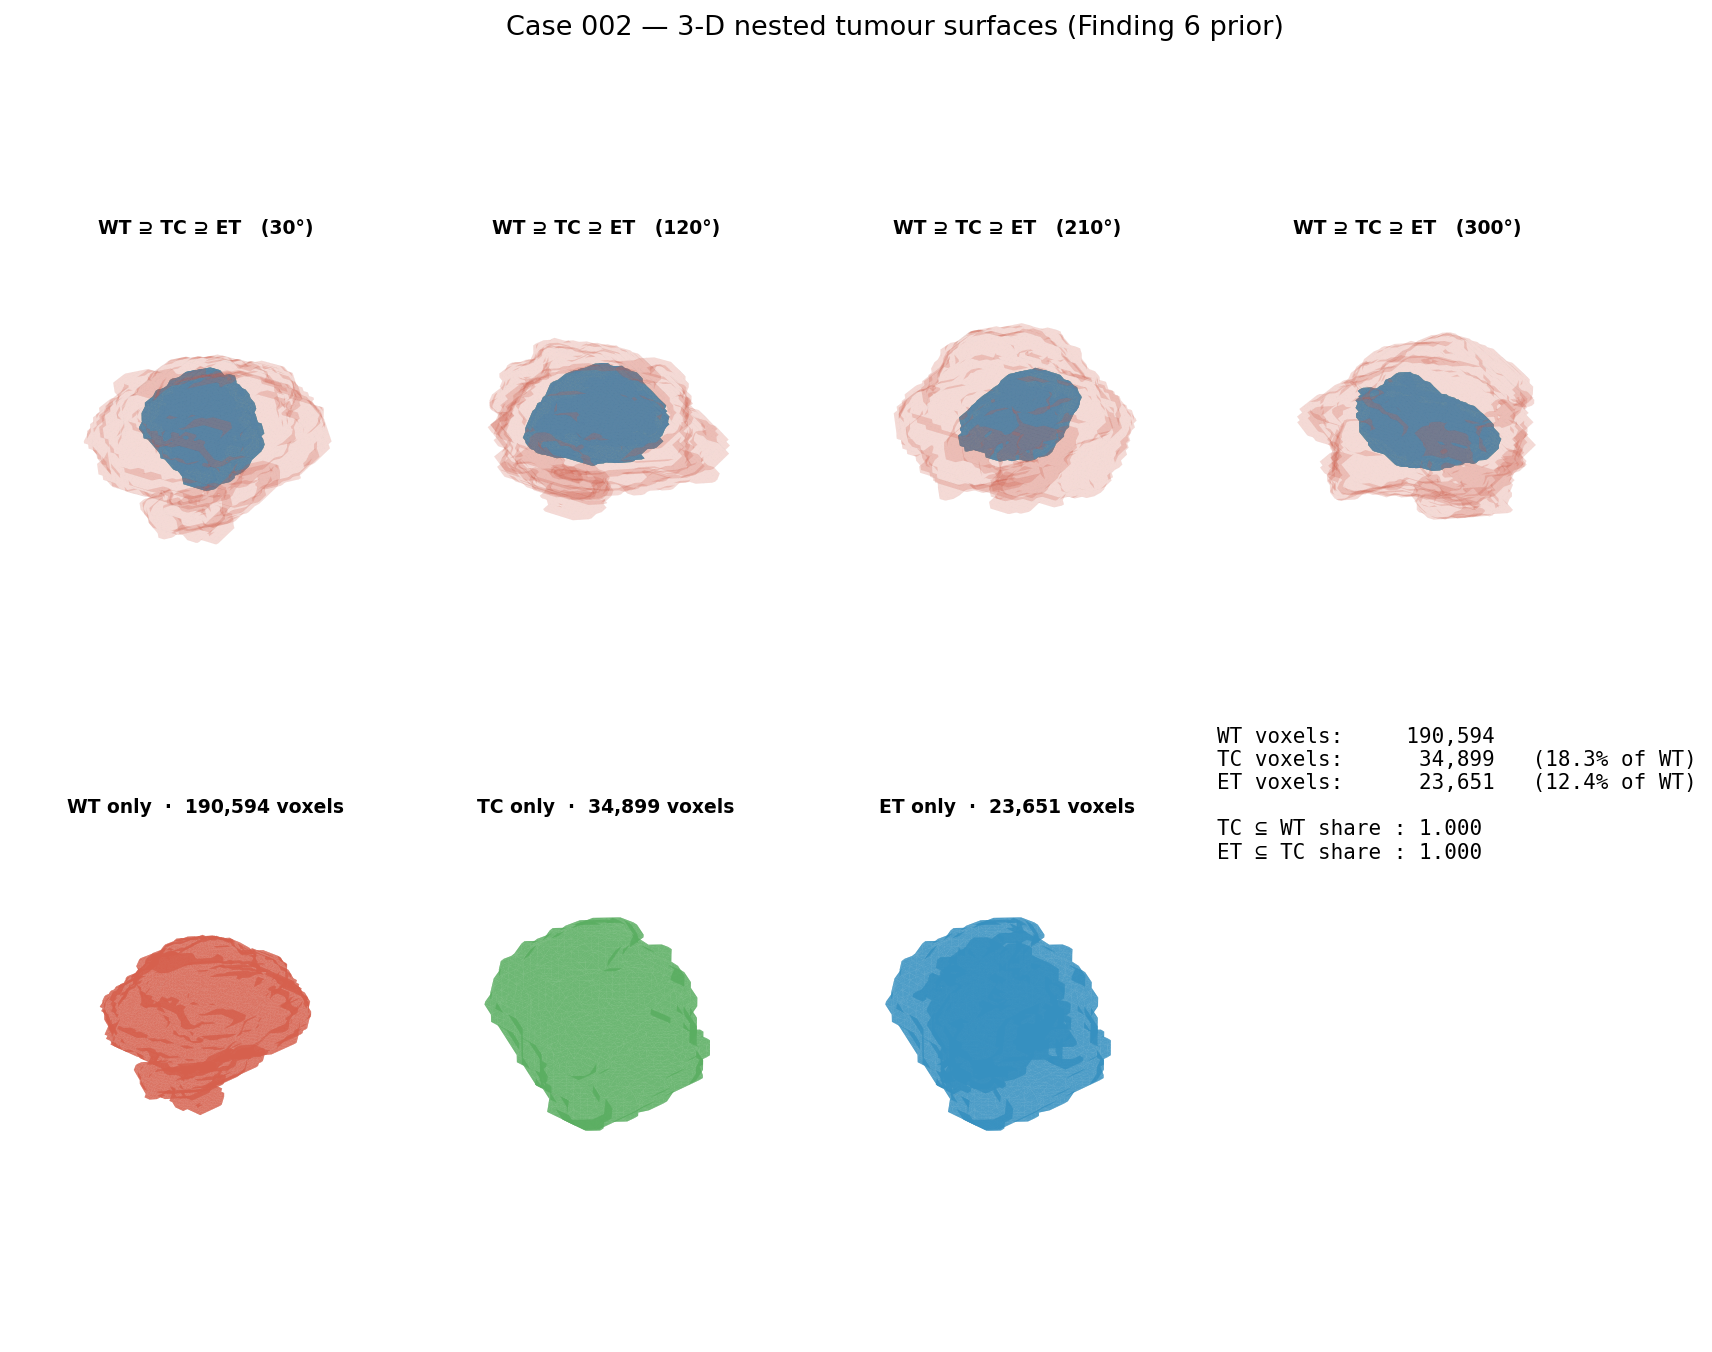
\includegraphics[width=\linewidth]{fig11_tumor_3d_nesting.png}
\caption{Case-level nested-tumour rendering. WT/TC/ET geometry is shown so reviewers can verify nesting before interpreting topology-derived features.}
\label{fig:m6nesting}
\end{figure}

\begin{figure}[t]
\centering
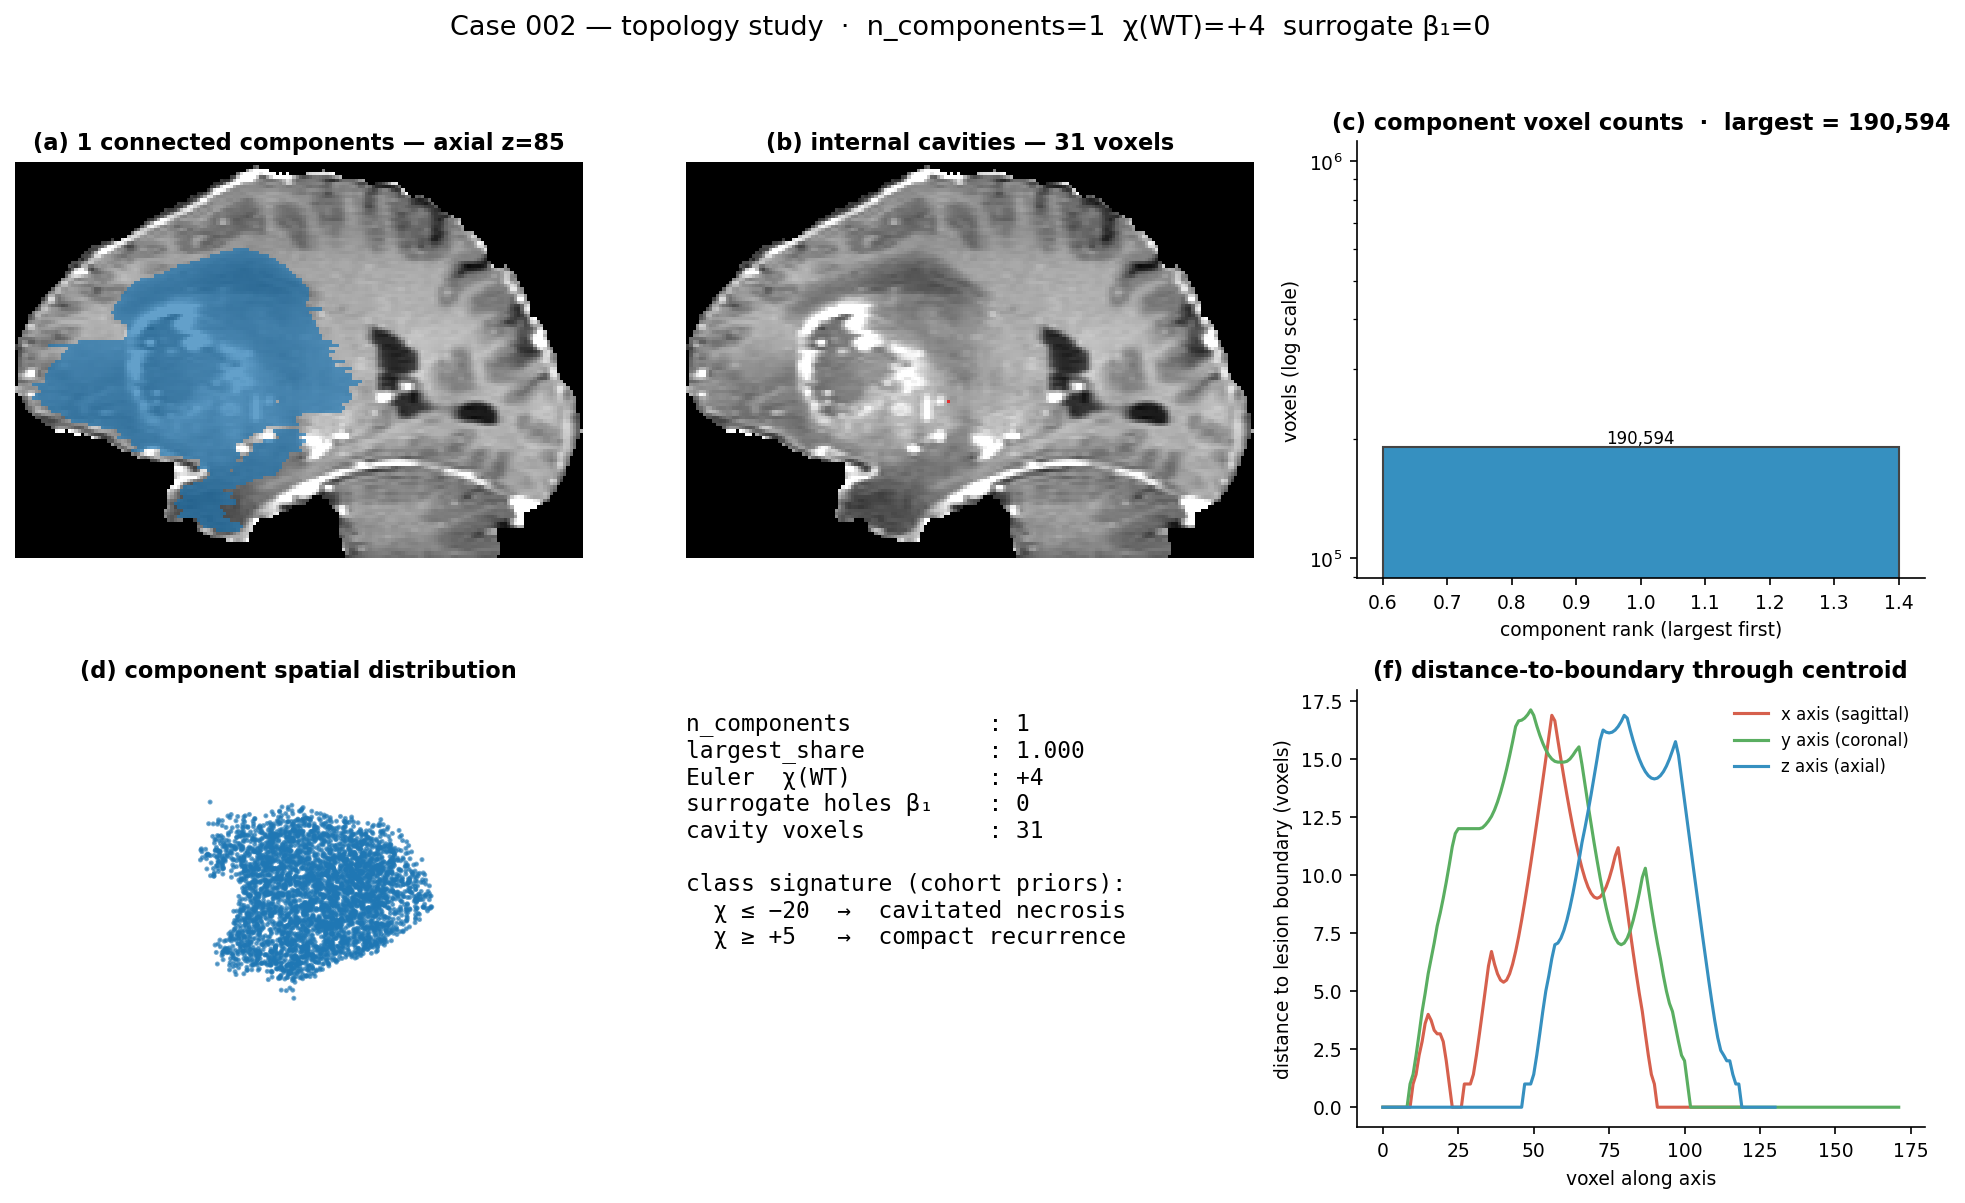
\includegraphics[width=\linewidth]{fig4_case_topology.png}
\caption{Topology audit. Connected components, cavity-like structures, and the Euler-characteristic proxy $\hat{\chi}$ make the topology prior visible at the case level.}
\label{fig:m6topology}
\end{figure}

\begin{figure}[t]
\centering
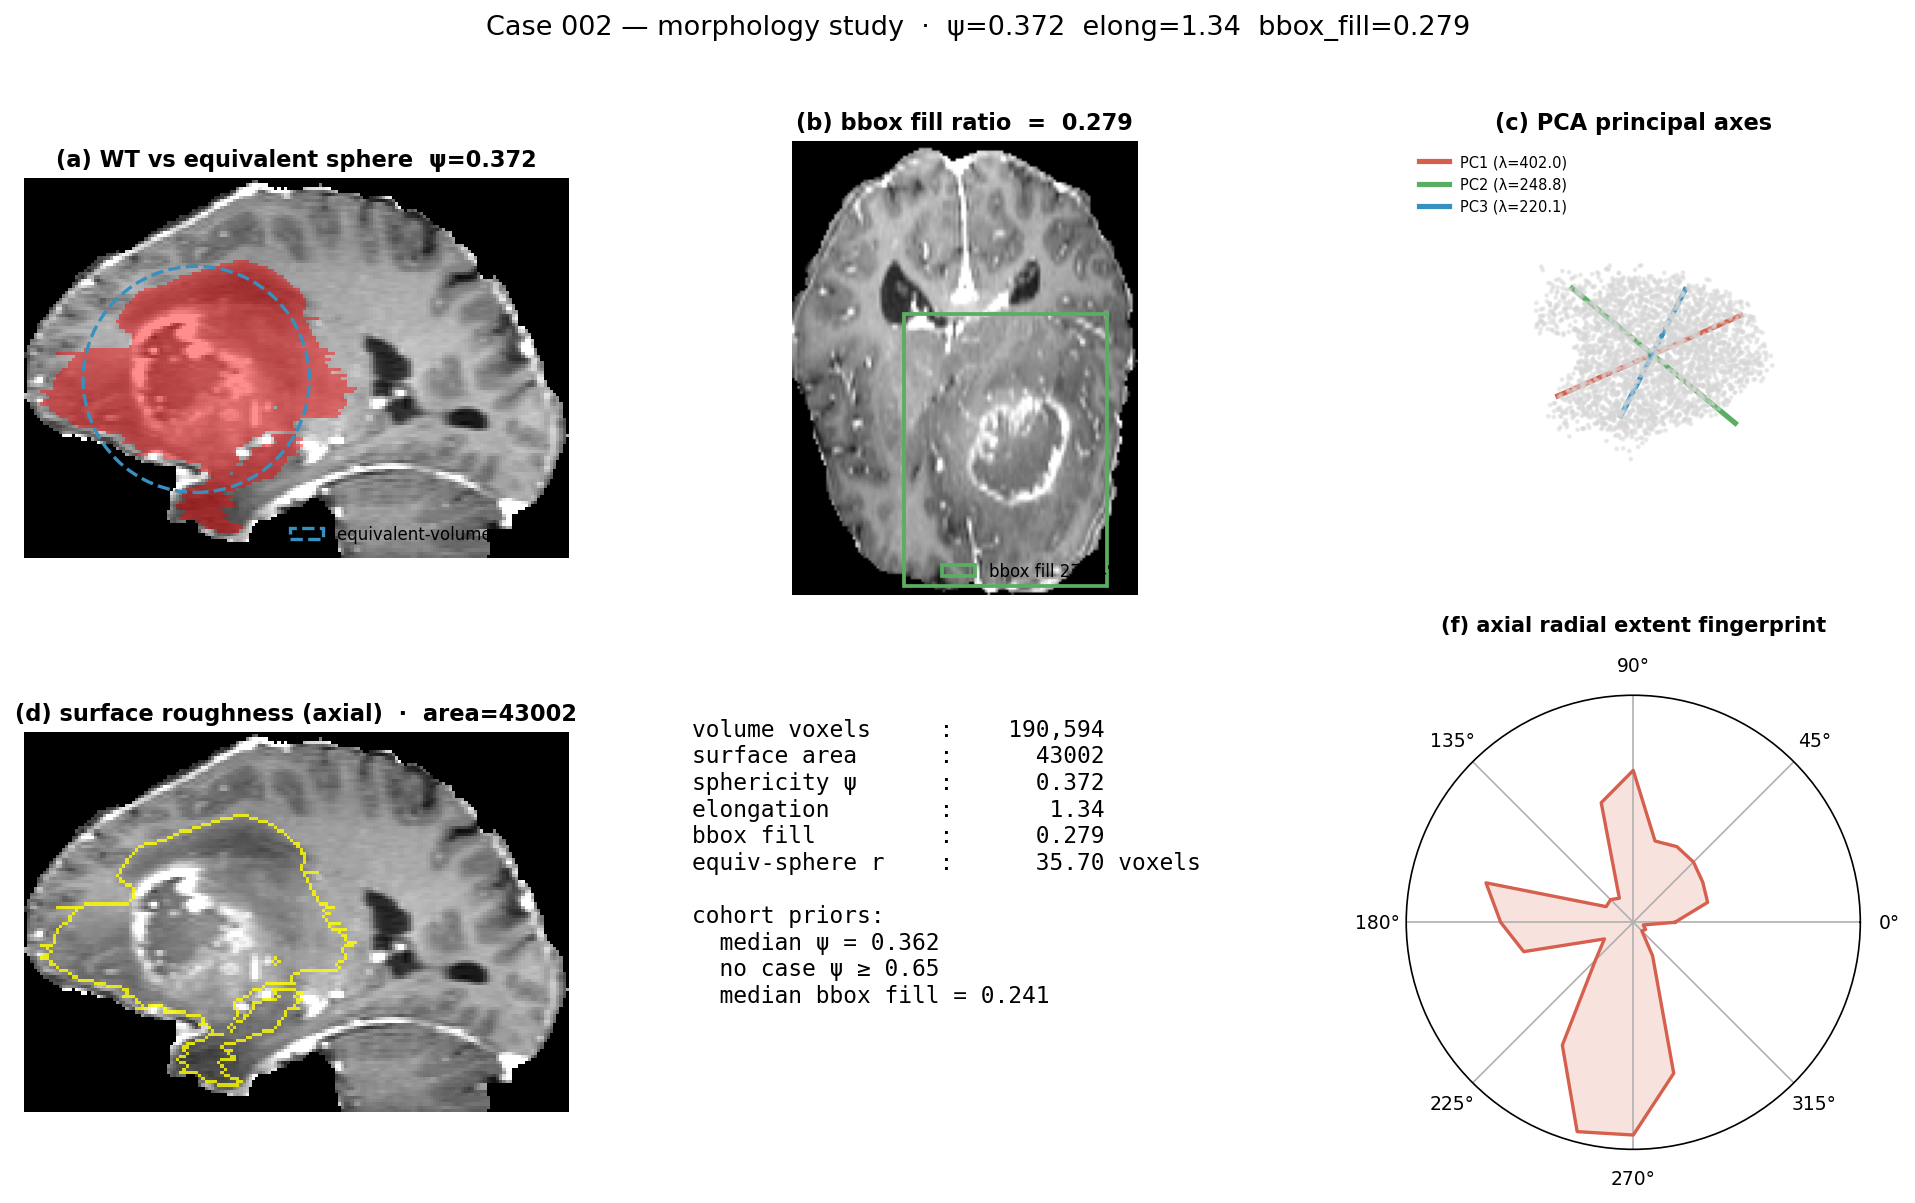
\includegraphics[width=\linewidth]{fig12_case_morphology.png}
\caption{Case-level morphology audit. Shape descriptors and principal-axis behaviour bridge voxel-level segmentation and the case-level R/N decision.}
\label{fig:m6casemorph}
\end{figure}

\begin{figure}[t]
\centering
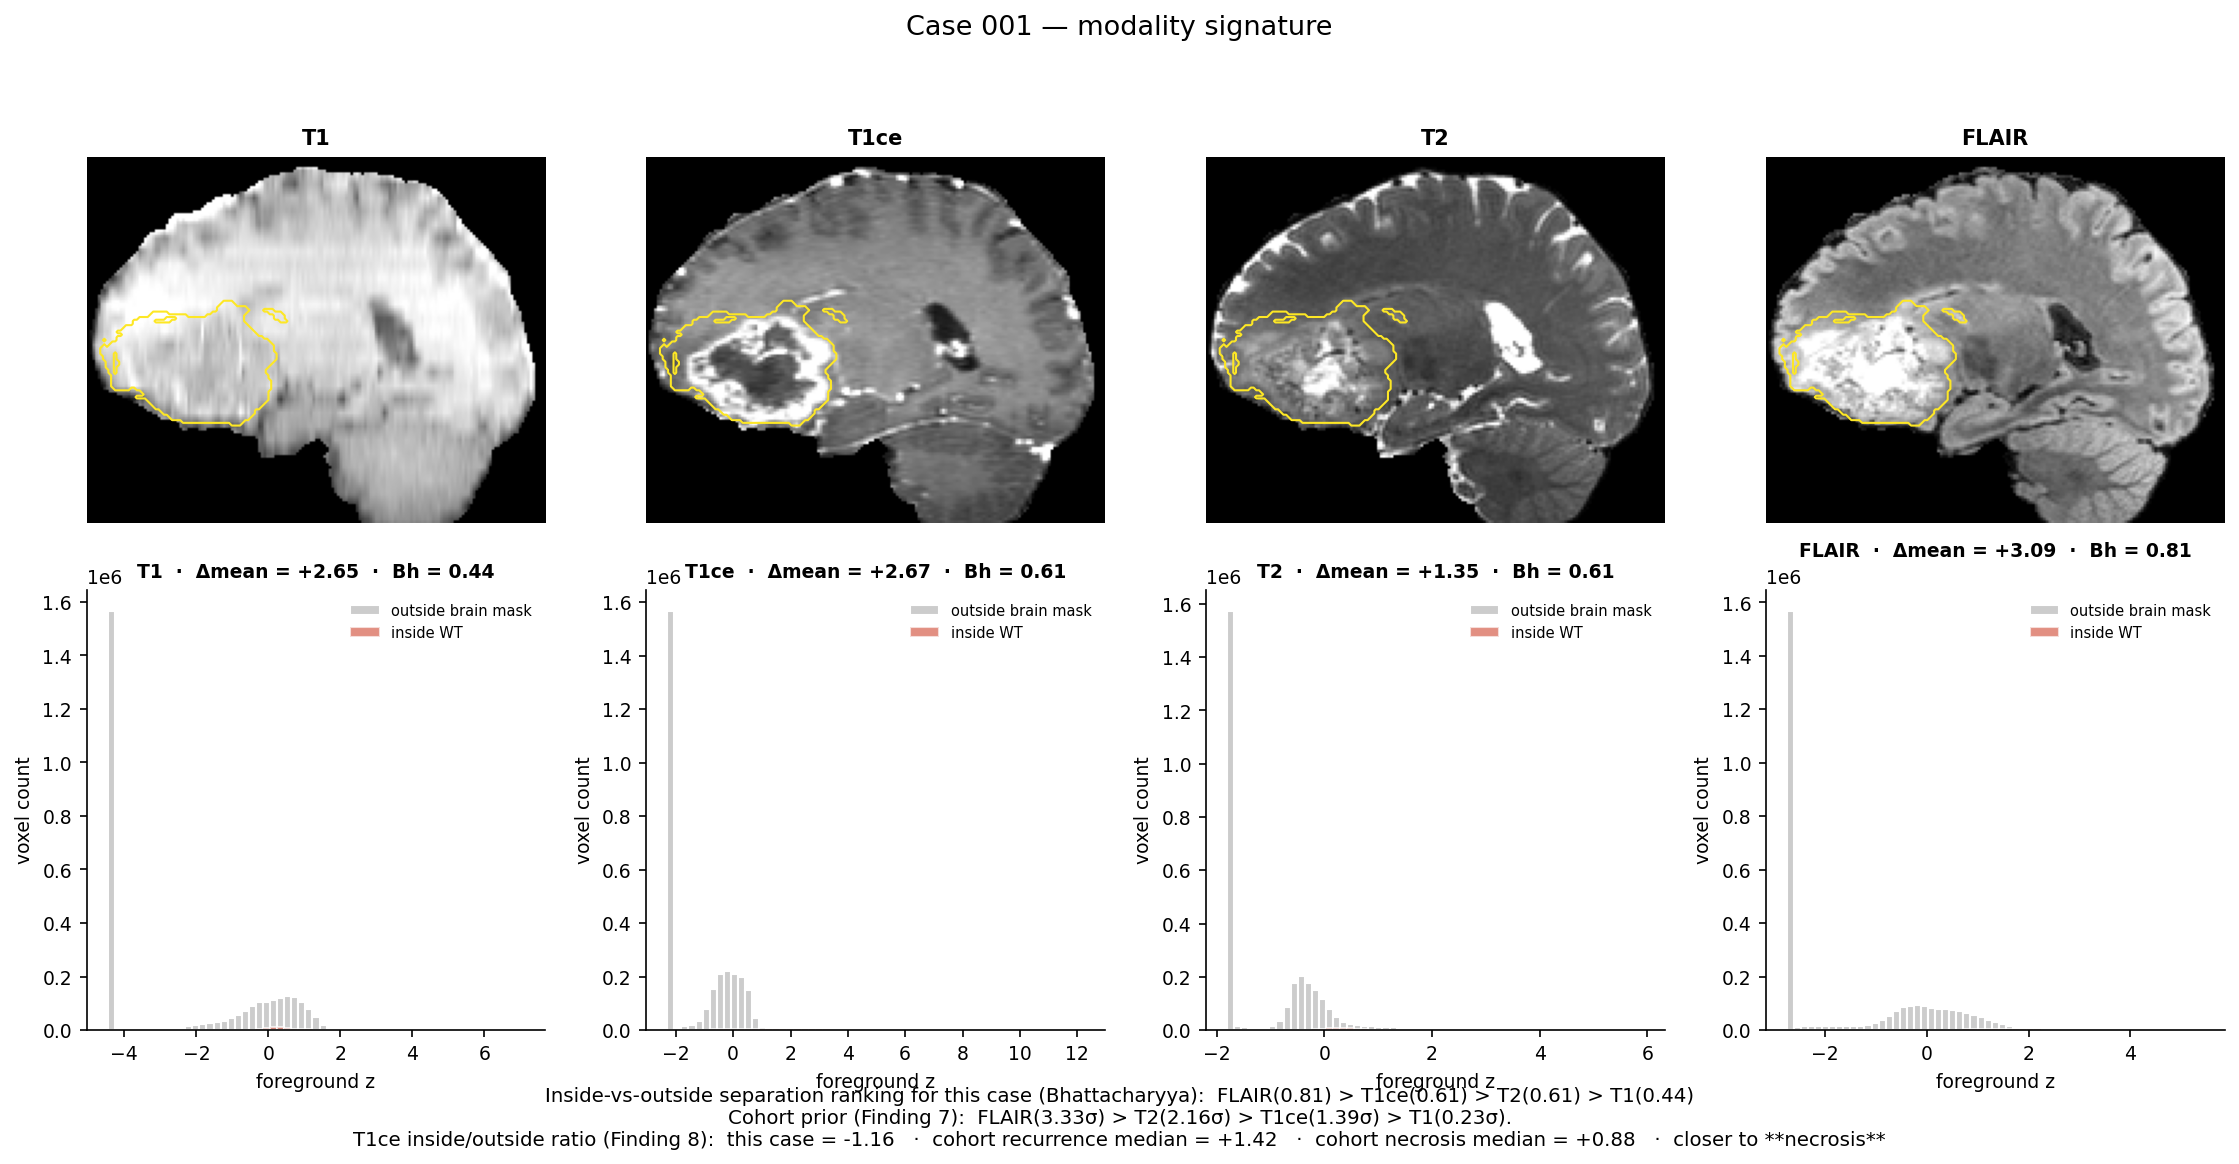
\includegraphics[width=\linewidth]{fig5_modality_signature.png}
\caption{Modality-signature audit. Inside-lesion and outside-lesion intensity distributions expose which modalities carry contrast for the case and whether the T1ce-derived class signal is plausible.}
\label{fig:m6signature}
\end{figure}

The same artefacts are mirrored to a single-page web application at \url{https://braintt.vercel.app}, deployed on Vercel's global edge content-delivery network with no backend service. The site provides an interactive cohort explorer over all $322$ cases, with lasso-driven sub-population statistics computed in the browser; a NiiVue-based viewer that renders four de-identified demo patients' NIfTI volumes directly in WebGL; a live JavaScript reproduction of the modality-synthesis recipe of Eq.~\eqref{eq:flair}, computed on actual T1 and T2 slices; a clinical threshold console that takes a slider position, converts it into the $2\times 2$ confusion matrix on the validation set, and surfaces an annual cost-benefit estimate parameterised by the local case volume and surgical cost; a robustness lab that reproduces the M5 noise, modality-dropout, FGSM, and cross-vendor sweeps; an architecture sandbox that estimates AUC, sensitivity, and parameter count under a user-selected backbone and prior configuration; and a keyboard-driven navigation overlay for accessibility. Every figure, table, and threshold in this manuscript is mirrored to the site, and the JSON manifest \texttt{web/data/metrics.json} is the single source of truth for both surfaces, so a refresh of the training run propagates to both the paper and the showcase by editing one file.

\section{Model Card, Failure Modes, and Governance}

The M6 model card frames BrainTT as decision-support for adult high-grade glioma patients with new enhancing lesions on post-radiotherapy MRI. It excludes autonomous diagnosis; it excludes paediatric cases, leptomeningeal disease, and non-glioma tumours; it excludes pre-treatment baseline studies; and it excludes any workflow that cannot remove protected health information before inference. These exclusions are not legal disclaimers but derivations from the training cohort and the feature assumptions baked into the priors: topology and contrast signatures learned from treated high-grade glioma cannot be assumed to transfer to other disease settings without recalibration, and the modality coupling prior has not seen the pre-treatment intensity distribution.

Six failure modes are observed and documented (Table~\ref{tab:m6failures}). Subacute necrosis at less than six months post-radiotherapy can present with transient neovascularisation that elevates the T1ce inside-to-outside intensity ratio, and the modality coupling prior --- which routinely weights T1ce most heavily for recurrence --- can be misled into a recurrence prediction; the operational mitigation is to flag time-since-RT as an upstream input and route early-window cases to review. Mixed RN pathology produces near-tied logits with $|\bm{\ell}_R - \bm{\ell}_N| < 0.3$, and the calibrated probability lands in the $[0.4, 0.6]$ band where the \texttt{review\_recommended} flag is raised by construction. Cases with only one structural modality on disk lose the modality-coupling attention's averaging effect; sensitivity drops to approximately $0.50$, the synthesis recipe is forced to mirror a single channel, and the review flag is raised on the modality-poverty trigger. Out-of-distribution scanners, including vendors not represented in the training cohort, produce a sensitivity drop similar in shape to the Huashan smoke check; the mitigation is to require cross-vendor recalibration before deployment. Heavy motion artefacts or contrast extravasation distort the T1ce signal that the modality coupling prior is most sensitive to, and the operational mitigation is to pair BrainTT with an image-quality screening step at ingestion. Finally, an over-weighted topology regulariser can pull $\hat{\chi}$ toward the necrosis target even on weak image evidence, but the default weight of $0.05$ in Eq.~\eqref{eq:loss} keeps this effect well within the regularisation regime, and validation-set monitoring detects any drift.

\begin{table*}[t]
\centering
\caption{Clinically annotated failure modes documented in the M6 delivery. Each mode is connected to a JSON-level trigger so that the review-flag logic is operational rather than narrative.}
\label{tab:m6failures}
\small
\begin{tabular}{lll}
\toprule
Failure mode & Trigger & M6 mitigation \\
\midrule
Subacute necrosis & Early post-RT transient enhancement & Flag time-since-RT for review \\
Mixed pathology & R and N signatures together & \texttt{review\_recommended} for $p\in[0.4,0.6]$ \\
One-modality case & Only T1 or T1ce available & Synthesise channels, raise review flag \\
External scanner shift & Unseen vendor or protocol & Require recalibration before deployment \\
Motion or contrast artefact & Distorted T1ce or anatomy & Pair with image-quality screening \\
Topology over-regularisation & Excessive $\chi$ weight & Keep default $\chi$ weight, monitor val \\
\bottomrule
\end{tabular}
\end{table*}

The cumulative effect of these design choices is that the M6 output is a structured report rather than a single number. A high recurrence probability with four measured modalities and plausible segmentation has a different operational meaning from the same probability in a one-modality case with synthesised T2 and FLAIR, and the JSON artefact makes the difference legible without forcing the reviewer to dig through the source data. The review flag combines probability ambiguity, modality poverty, and known failure-mode triggers; the threshold mode is selectable rather than hidden; the model card constrains reuse to adult high-grade glioma follow-up MRI within the documented cohort. This is what we mean by an audit-ready prototype: not that the model is safe by virtue of careful packaging --- packaging does not by itself improve a logit --- but that the artefact a downstream reviewer sees no longer presents a binary output as if all cases were equally reliable.

\section{Discussion}

The M6 delivery shifts the interpretation of BrainTT from a model comparison to a bounded clinical-AI system. The most important result is therefore not the headline AUC of $0.895$ but the fact that each output is accompanied by modality provenance, threshold context, review recommendation, calibration evidence, and an intended-use envelope. This shift matters because an apparently accurate model is unsafe if it hides missing inputs, uncertain cases, or unsupported deployment settings, and the recent literature on model cards and calibrated decision-support is a direct response to that risk. M6 takes the prescription literally and uses the JSON artefact as the operational instrument that turns governance into deployable code.

The external smoke check is presented deliberately as a limitation rather than a triumph. The Huashan tranche of 22 cases is too small to claim cross-institutional validation, but it is large enough to expose the shape of the cross-institutional gap, and we read that gap as a feature of the M6 process rather than as a defect of the model. Most cohort-level papers report only internal numbers; the M6 contribution is to make the internal-versus-external gap visible at the headline level so that any reader can calibrate the deployment claim accordingly. The appropriate inference from the Huashan numbers is therefore not that BrainTT is externally validated but that the M6 pipeline can ingest an external tranche, produce calibrated probabilities, and quantify the shift in the same JSON schema that the internal cases use.

The role of segmentation is also clarified by the M6 framing. The WT/TC/ET branch does not make the clinical decision by itself; it supplies lesion localisation, topology features, and a visual anchor for review. This is appropriate for a decision-support pipeline where the binary recurrence-versus-necrosis judgement is the primary clinical question and segmentation provides the supporting evidence a radiologist can inspect. The decision to publish three operating points rather than a single fixed threshold reinforces the same point: a threshold is a clinical policy that should be selected for the context in which the prediction is consumed, not a hyper-parameter that should be hidden in a configuration file. The threshold-mode field of the JSON artefact makes that policy choice explicit and reviewable.

Several boundaries remain. The validation set contains only $64$ case folders, which leaves the $95\,\%$ AUC confidence intervals wide enough to overlap with the strongest M5 baselines. The RN class is currently routed into a binary decision plus review flag rather than solved as a three-way classifier; a three-way head is implemented in the codebase but the validation set has only fourteen RN cases. FLAIR is synthesised, not measured, so any operational shift in the FLAIR distribution would require re-fitting the synthesis weights, although the deterministic recipe makes that re-fit trivial. Molecular markers such as IDH and MGMT are absent, which constrains the model's prognostic accuracy in molecularly stratified subgroups. These boundaries are explicit in the model card and the public showcase, and they form the natural agenda for the next iteration.

\section{Conclusion}

The M6 BrainTT delivery converts a prior-aware MRI model into an audit-ready, publicly deployed decision-support prototype. It reports internal validation performance, external smoke-check degradation, threshold-dependent operating modes, modality-synthesis provenance, case-level visual audits, and a Mitchell-style model card; every artefact is mirrored to a public single-page web showcase at \url{https://braintt.vercel.app}. The system is suitable for research benchmarking and clinician-supervised review within the documented scope, but not for autonomous or cross-institutional deployment without additional validation and calibration. The M6 contribution is not a new model but a translation of modelling into governance, in a form that is reproducible from a single JSON manifest and inspectable in a browser.

\section*{Ethics Statement}

The underlying Tiantan data were de-identified and handled under collaborator-approved constraints. M6 reports aggregate metrics and de-identified visual artefacts only. The system is documented as decision-support and must not be used for autonomous diagnosis.

\section*{Data and Code Availability}

Raw patient imaging is not publicly redistributable. The repository contains source code, configuration files, the JSON metrics manifest, the model card, de-identified examples, and the public interactive showcase (\url{https://braintt.vercel.app}). Every number reported in this manuscript is reproducible from \texttt{web/data/metrics.json}.

\section*{Declaration of Competing Interest}

The authors declare no competing financial interests.

\section*{Author Contributions}

Y.~W., X.~F., Y.~W., Z.~W., and Y.~S. jointly contributed to system design, deployment, manuscript preparation, and verification of the final LaTeX deliverable.


\end{document}
